\chapter{Conclusion}
\label{chapter:Conclusion}

Dans ce chapitre, nous effectuons une synthèses des contributions proposées dans cette thèse, nous rappelons les cas d'usages possibles, et nous discutons des menaces de validité.
Nous proposons ensuite plusieurs perspectives, dont une extension succinctement testée de la méthode CREA pour pouvoir prendre en compte l'axe temporel et ordonnancer les clusters.


\bigskip

\minitoc % Creating an actual minitoc / ToC local to a chapter

\newpage

%%%%%%%%%%%%%%%%%%%%%%%%%%%%%%%%%%%%%%%%%%%%%%%%%%%%%%%%%

\section{Synthèse}
\label{section:Conclusion:Synthese}

Dans cette thèse nous avons étudié la question de la réutilisation et de la pertinence du contexte dans le cadre de la gestion des connaissances et des processus à forte intensité de connaissances.
Nous avons conçu et implémenté la méthode CREA permettant de réutiliser des documents existants afin de proposer des séances constituées de plusieurs notions à un enseignant.
Cette méthode peut également être utilisée à d'autres fins comme vérifier la pertinence des documents vis-à-vis d'un sujet ou visualiser graphiquement les mots clés d'un corpus documentaire.


\subsection{Rappel des contributions}
\label{subsection:Conclusion:Synthese:RappelContributions}

La méthode CREA, \MyCREA, vise à permettre de réutiliser des supports de cours et autres documents existants afin de proposer des ensembles de termes sous forme de séances, tout en s'assurant de la pertinence des documents sélectionnés.
Pour cela, la méthode CREA s'appuie tout d'abord sur un pré-traitement sémantique des documents afin d'en extraire les notions les plus pertinentes pour l'enseignant sous forme de concepts et d'entités nommées issus du réseau sémantique BabelNet.
Le résultat de ce pré-traitement sémantique permet ensuite d'effectuer des analyses plus poussées sur deux métriques en s'appuyant sur les liens entre les documents et les termes illustrant une partie des connaissances tacites exploitées par les auteurs desdits documents.

\bigskip

Afin de sélectionner les documents les plus adaptés, une première contribution concerne la visualisation des notions retrouvées dans l'ensemble du corpus documentaire et la pertinence des documents par rapport aux notions clés retrouvées.
Le graphe illustré par la figure~\ref{figure:5-GrapheCoreZoom} permet à un enseignant de visualiser les notions les plus importantes dans son corpus documentaire (les n\oe{}uds rouges et oranges dans cet exemple), mais également la pertinence des documents (les n\oe{}uds gris indiquant la référence du document) sous forme de distance des uns par rapport aux autres et à l'ensemble central de notions.
Cette cartographie s'appuie sur l'analyse de concepts formels et l'impact mutuel afin de comprendre les relations entre les termes précédemment extraits et les documents les contenant.

\bigskip

L'enseignant se voit proposer plusieurs séances, et les notions à aborder dans chacune d'elle, à l'issue de plusieurs traitements.
Ces séances sont représentées sous forme de clusters de termes comme illustré par la figure~\ref{figure:5-ClustersStrategieHauteBeta1}.
Pour cela, nous avons utilisé la stratégie haute de binarisation, l'analyse de concepts formels, le calcul de la similarité conceptuelle, et la classification ascendante hiérarchique afin d'obtenir des regroupements issus des termes les plus fréquents du corpus documentaire.
Les clusters générés ne sont pas encore organisés temporellement et restent une proposition que l'enseignant peut encore adapter à son cas.

% ESTHETIQUE
\newpage

\hspace{0pt}
\vfill


\begin{figure}[htb!]
\centering
\centerline{  % FORCE FIGURE OUTSIDE THE MARGIN !!! BUT STILL CENTERING !!!
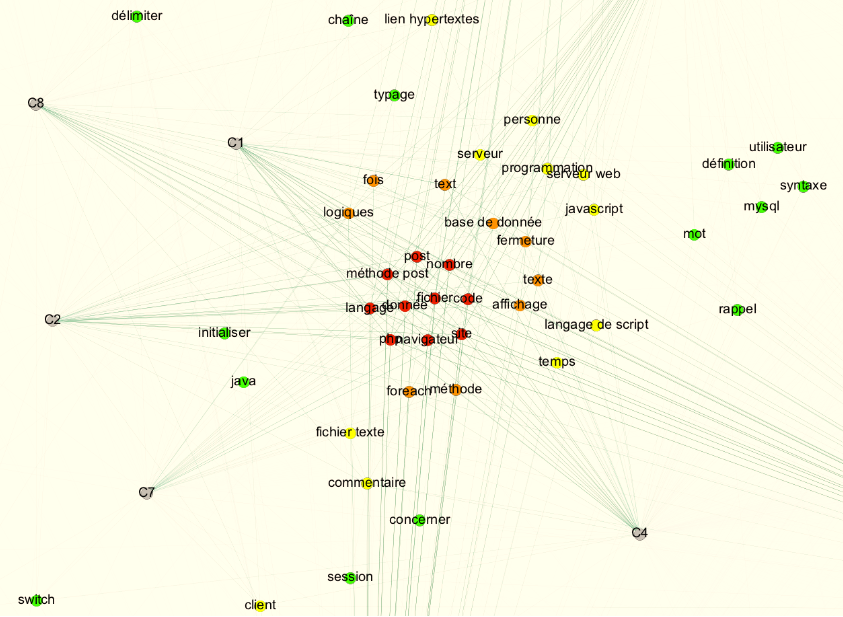
\includegraphics[scale=0.65]{4-Experiences/images/cas-1/graphe-Directe-core-zoom.png}
}
\caption{Graphe d'impact mutuel : notions centrales et documents}
\label{figure:5-GrapheCoreZoom}
\end{figure}



\begin{figure}[htb!]
\centering
\centerline{  % FORCE FIGURE OUTSIDE THE MARGIN !!! BUT STILL CENTERING !!!
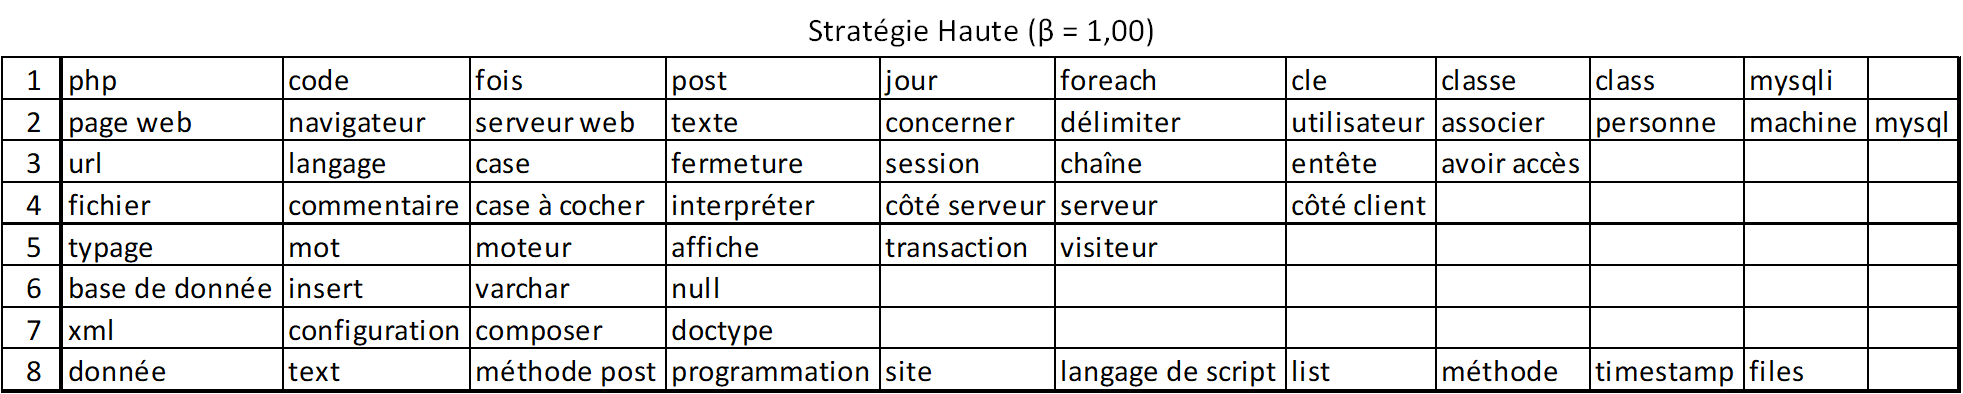
\includegraphics[scale=0.65]{4-Experiences/images/cas-1/clusters-S=H-B=1.00.png}
}
\caption{Clusters de termes : proposition de découpage en séances}
\label{figure:5-ClustersStrategieHauteBeta1}
\end{figure}

\vfill
\hspace{0pt}

%\newpage
% FIN ESTHETIQUE



%%%%%%%%%%%%%%%%%%%%%%%%%%%%%%%%%%%%%%%%%%%%
\clearpage % Clean for pictures and tables %
\newpage   % Clean for pictures and tables %
%%%%%%%%%%%%%%%%%%%%%%%%%%%%%%%%%%%%%%%%%%%%

%%%%%%%%%%%%%%%%%%%%%%%%%%%%%%%%%%%%%%%%%%%%%%%%%%%%%%%%%

\subsection{Usages possibles}
\label{subsection:Conclusion:Synthese:Usages}

La méthode CREA vise à guider un enseignant dans la conception d'un nouveau cours en proposant des clusters de notions issus de supports de cours existants, le tout en s'appuyant sur de nombreux outils automatiques.
Cependant, d'autres cas d'usages s'appuyant sur la réutilisation en découlent également.

\bigskip

La méthode nécessite de réunir des supports de cours contenant du texte, et d'indiquer le nombre de séances voulues.
Les supports insérés sont tout d'abord traités par plusieurs techniques de traitement automatique du langage pour en extraire des termes illustrant les notions abordées.
Puis, une combinaison d'analyse de concepts formels et de clustering permet d'en extraire un graphe représentant les termes les plus représentatifs du corpus, la pertinence des documents de ce corpus, ainsi que des clusters regroupant les termes réutilisables par l'enseignant.
L'enseignant obtient ainsi plusieurs ensembles de termes liés à partir desquels il peut construire son propre cours selon ses attentes et exigences.

\bigskip

Afin d'améliorer la qualité, un enseignant peut éliminer des documents isolés dans le graphe d'impact mutuel et relancer la méthode, ou raffiner manuellement les termes entre chacune des étapes de la méthode.
Une contrainte imposant d'éliminer certains termes peut également être appliquée en supprimant ces termes durant les traitements, ou en retirant les documents contenant ces termes.

Un enseignant souhaitant obtenir une liste de termes clés d'un domaine peut donc s'appuyer sur le graphe d'impact mutuel généré par plusieurs documents représentant ce domaine.
Les cas d'usages peuvent concrètement être vus ainsi :

\begin{enumerate}
\item Construction d'un nouveau cours à partir d'anciens cours
	\begin{itemize}
	\item Entrées : \textit{Documents} (supports de cours d'autres enseignants),
					\textit{Nombre de séances}
	\item Sorties : \textit{Graphe d'impact mutuel} (cartographie des notions du corpus documentaire, et pertinence des documents),
					\textit{Clusters de notions} (organisation des notions sous formes d'autant de séances que demandées)
	\end{itemize}

\item Comparaison de son propre cours par rapport à d'autres cours et aux productions académiques
	\begin{itemize}
	\item Entrées : \textit{Documents} (son propre support de cours + supports de cours d'autres enseignants, articles de recherche, livres, ...)
	\item Sorties : \textit{Graphe d'impact mutuel} (cartographie des notions du corpus documentaire, et positionnement de son propre cours parmi les autres documents)
	\end{itemize}

\item Découverte d'un domaine académique
	\begin{itemize}
	\item Entrées : \textit{Documents} (articles de recherche, livres, ...), \textit{Paramètres des stratégies} (choix de la stratégie directe, haute, ou moyenne, et choix du $ \beta $ selon la granularité visée)
	\item Sorties : \textit{Graphe d'impact mutuel} (cartographie des notions du corpus documentaire)
	\end{itemize}

\item Filtrage d'un corpus documentaire pour ne garder (ou retirer) que les documents traitant de certains thèmes précis
	\begin{itemize}
	\item Entrées : \textit{Documents}, \textit{Notions et termes recherchés}
	\item Sorties : \textit{Graphe d'impact mutuel} (cartographie des liens entre les termes et les documents)
	\end{itemize}

\item Aide à la composition de l'index d'un ouvrage
	\begin{itemize}
	\item Entrées : \textit{Document(s)}, \textit{L'ouvrage rédigé, éventuellement les principales sources utilisées ou les plus influentes}
	\item Sorties : \textit{Liste de termes} (liste issue du pré-traitement sémantique, voire, filtrée suite à la stratégie haute de binarisation)
	\end{itemize}

\end{enumerate}

\bigskip

Au delà du domaine d'application de l'enseignement supérieur et de la recherche, la visualisation de la pertinence des documents peut être utilisée dans les situations où la sélection de documents basée sur les concepts et termes employés est requise, de même pour la visualisation des sujets abordés dans un ensemble documentaire.
La prise de décision basée sur la pertinence de documents, l'absence/présence de termes dans ces derniers, ou les sujets d'intérêts d'un corpus documentaire grâce à la première contribution de la méthode CREA est donc tout à fait réaliste.
À l'inverse, l'organisation sous forme de clusters des termes avec le fonctionnement actuel ne semblent pas transposable à d'autres usages contemporains : rechercher les maladies causant certains symptômes nécessite des traitements supplémentaires pour obtenir des clusters regroupant les combinaisons utiles, par exemple.
Un usage original des premières étapes de la méthode consiste à aider un auteur en recherchant les termes clés dans son ouvrage, et éventuellement des sources qu'il utilise, afin de lui suggérer des mots-clés pour son index.
La simple recherche de noms ou de verbes génèrera une liste particulièrement longue, mais BabelFy couplé à la stratégie de binarisation peuvent déterminer quels termes et concepts sont les plus appropriés.
La méthode CREA dans son ensemble est donc actuellement dédiée à un usage appliqué à l'enseignement supérieur et à la recherche.

%%%%%%%%%%%%%%%%%%%%%%%%%%%%%%%%%%%%%%%%%%%%
\clearpage % Clean for pictures and tables %
\newpage   % Clean for pictures and tables %
%%%%%%%%%%%%%%%%%%%%%%%%%%%%%%%%%%%%%%%%%%%%

%%%%%%%%%%%%%%%%%%%%%%%%%%%%%%%%%%%%%%%%%%%%%%%%%%%%%%%%%

\subsection{Menaces de validité}
\label{subsection:Conclusion:Synthese:MenacesValidite}

Sept types de menaces de validité sont présentés dans~\cite{feldt2010validity} : validité de la conclusion, validité interne, validité de la construction, validité externe et transférabilité, crédibilité, fiabilité, et confirmation.

\bigskip

La validité de conclusion concerne la mesure de changements significatifs dans les résultats grâce à l'usage de notre artefact.
Étant donné que la méthode CREA n'a pas été comparée à d'autres méthodes traitant du même sujet, et qu'elle ne produit pas un cours en entier, ce type de validité est difficile à vérifier.
Comme nous l'avons précédemment vu, la comparaison des partitions n'a pas donné de résultat satisfaisant de par la nature des termes et clusters manipulés : la combinaison de termes implique une interprétation avec un contexte.
La comparaison des résultats produits par un humain variera indéniablement selon la personne qui fera l'évaluation et son niveau d'expertise (qui évolue lui aussi au cours du temps).
Il est donc possible qu'une même personne n'ait pas le même avis sur les mêmes résultats produits à plusieurs instants différents.

\bigskip

La validité interne concerne les facteurs ayant un impact sur les résultats produits par l'artefact.
Dans notre cas, nous avons étudié ces limites grâce aux différentes validations structurelles, puis nous avons discuté des différents problèmes lors des discussions.
Typiquement, les types de documents (format diapositive ou texte) ont un impact sur les graphes d'impact mutuel, mais également sur la quantité de termes dans les clusters de sortie.
Il est nécessaire de chercher à limiter le nombre de termes, voire, de remonter plus en amont et comprendre les relations entre le nombre de documents, la quantité de termes contenus, la valeur de $ \beta $, et le nombre de clusters.

\bigskip

La validité de la construction s'intéresse au phénomène que l'artefact est censé traiter, ainsi qu'aux effets impactant les résultats.
Nous nous sommes intéressés à la réutilisation des connaissances dans le cadre de la construction de cours, et nous avons effectivement constaté que les connaissances tacites ont un effet sur l'interprétation des résultats.
Les différentes étapes de la méthode CREA visent à reproduire certaines manipulations humaines (extraire le sujet central des documents, indiquer quel document est hors sujet, etc) et produisent des résultats intéressants qui peuvent être encore améliorés.
Nous avons bel et bien été confrontés aux difficultés liées aux connaissances tacites, tout en faisant une extraction et des filtrages pertinents concernant les termes.
Notre artefact est donc valide de ce point de vue.

\bigskip

La validité externe et la transférabilité concernent la généralisation dans d'autres cas et situations.
La généralisation (du point de vue fonctionnel) à l'ensemble des domaines d'études, voire, à l'ensemble des processus à forte intensité de connaissances n'a pas été démontrée.
On peut tout de même supposer que BabelFy s'appuyant sur des bases de connaissances larges, tous les sujets seront probablement pris en charge tant qu'ils sont suffisamment documentés, mais nous ne pouvons pas l'assurer.
Des scénarios touchant à des domaines moins industriels et beaucoup plus académiques pourraient être testés et évalués avec des experts du domaine (au lieu de PHP ou de \textit{statecharts}, des documents traitant de philosophie pourraient être testés).

En dehors du cadre de la construction de cours, nous n'avons ni testé l'utilisation d'autres bases de connaissances plus spécifiques à l'industrie, ni l'ensemble des cas d'usages précédemment présentés.

\bigskip

La généralisation (du point de vue plus technique) à n'importe quel scénario n'est pas non plus démontrée.
Les scénarios testés dans cette thèse ont permis d'achever plusieurs essais ouvrant une voie intéressante, mais pas totalement validée.
En effet, la quantité de documents en entrée semble impacter les résultats et ne permet pas de totalement confirmer les hypothèses traitant des types de documents.
Des scénarios testant tout d'abord uniquement des supports de cours sur un sujet actuellement maîtrisé, puis uniquement sur les articles de recherche ayant mené au développement et à la maturité de ce sujet permettraient de mieux observer les effets sur les graphes d'impact mutuel et les clusters résultant.

Ces scénarios souffrent néanmoins de l'évolution du vocabulaire au cours du temps : un sujet ayant mis plusieurs années à arriver auprès du grand public peut avoir vu énormément d'évolution dans son vocabulaire, dont certains termes pourraient être réutilisés dans un autre contexte proche (et donc avoir une autre définition), ou avoir tout simplement disparu.
Par exemple, les \og \textit{moniteurs transactionnels} \fg (permettant de traiter des transactions) n'ayant plus exactement d'existence dans les systèmes classiques actuels (car intégrés aux \og \textit{systèmes de gestion de bases de données} \fg et à leurs \og \textit{connecteurs} \fg), leur mention dans les articles, ouvrages, ou anciens supports de cours ne sera pas toujours comprise par le lecteur, voire, la création de liens sémantiques sera plus complexe si la définition n'est pas parfaitement déclarée dans la base de connaissances.

Des scénarios utilisant des supports de cours récents sur un sujet contemporain, en comparant leurs résultats par rapport à ceux d'articles de recherche, pourraient être corrects.
Il faut néanmoins s'assurer que les supports de cours respectent les exigences concernant la quantité minimale de texte.
On peut également poser la question sur la construction de ces supports : étant donné qu'ils sont déjà des résumés des articles, ils pourraient tout simplement servir à confirmer la structure produite par la méthode CREA à partir des articles.

Concernant la langue des documents, nous n'avons pas testé au sein d'un même scénario l'usage de plusieurs langues distinctes.
BabelFy permet déjà de retrouver un concept quel que soit sa langue, mais l'ensemble du document doit être dans la même langue (ou alors il faut manuellement tagger les mots).
Bien qu'il semble très probable qu'un tel scénario produise des résultats corrects, une confirmation pratique pourrait être utile.

\bigskip

La crédibilité concerne la confiance dans les conclusions trouvées.
La démarche effectuée étant inspirée du design science, plusieurs expériences ont permis d'affiner les résultats et mieux comprendre l'origine de certaines anomalies (par exemple l'impact de la taille des documents sur les graphes d'impact mutuel).
Les expériences successives ont permis d'observer des améliorations notables lors de corrections, et indiquer des facteurs à surveiller à l'avenir.

\bigskip

La fiabilité concerne la cohérence des résultats.
Comme nous l'avons expliqué, une confiance absolue dans la méthode CREA est actuellement impossible, mais les résultats actuels et les fondements théoriques des outils utilisés indiquent des cas où les résultats sont cohérents et peuvent être consolidés avec d'autres recherches plus approfondies.
Les graphes d'impact mutuel affichent des résultats cohérents et pertinents, et les facteurs les impactant sont de mieux en mieux identifiés.
Les clusters nécessitent quant à eux d'autres travaux.

\bigskip

Enfin, la confirmation vise à connaître à quel point les conclusions ont été façonnés par les résultats d'expériences plutôt que par le chercheur et ses biais ou intérêts.
L'interprétation des résultats s'appuyant totalement sur nos connaissances tacites, un biais existe.
Afin de limiter ce biais, d'autres informaticiens ont également évalué une partie du cas de référence afin de déterminer si ces résultats sont cohérents.
Bien qu'il soit impossible d'éviter certains biais d'interprétation, l'objectif de simplifier la lecture d'un corpus documentaire volumineux lors de la construction d'un cours est une motivation très intéressante pour l'ensemble des enseignants-chercheurs.


%\bigskip


%%%%%%%%%%%%%%%%%%%%%%%%%%%%%%%%%%%%%%%%%%%%%%%%%%%%%%%%%%%%%%%%%%%%%%%%%%%%%%%%%%%%%%%%%%
%%%%%%%%%%%%%%%%%%%%%%%%%%%%%%%%%%%%%%%%%%%%%%%%%%%%%%%%%%%%%%%%%%%%%%%%%%%%%%%%%%%%%%%%%%
%%%%%%%%%%%%%%%%%%%%%%%%%%%%%%%%%%%%%%%%%%%%%%%%%%%%%%%%%%%%%%%%%%%%%%%%%%%%%%%%%%%%%%%%%%
%%%%%%%%%%%%%%%%%%%%%%%%%%%%%%%%%%%%%%%%%%%%%%%%%%%%%%%%%%%%%%%%%%%%%%%%%%%%%%%%%%%%%%%%%%
%%%%%%%%%%%%%%%%%%%%%%%%%%%%%%%%%%%%%%%%%%%%%%%%%%%%%%%%%%%%%%%%%%%%%%%%%%%%%%%%%%%%%%%%%%
%%%%%%%%%%%%%%%%%%%%%%%%%%%%%%%%%%%%%%%%%%%%%%%%%%%%%%%%%%%%%%%%%%%%%%%%%%%%%%%%%%%%%%%%%%

%%%%%%%%%%%%%%%%%%%%%%%%%%%%%%%%%%%%%%%%%%%%
\clearpage % Clean for pictures and tables %
\newpage   % Clean for pictures and tables %
%%%%%%%%%%%%%%%%%%%%%%%%%%%%%%%%%%%%%%%%%%%%

%%%%%%%%%%%%%%%%%%%%%%%%%%%%%%%%%%%%%%%%%%%%%%%%%%%%%%%%%%%%%%%%%%%%%%%%%%%%%%%%%%%%%%%%%%
%%%%%%%%%%%%%%%%%%%%%%%%%%%%%%%%%%%%%%%%%%%%%%%%%%%%%%%%%%%%%%%%%%%%%%%%%%%%%%%%%%%%%%%%%%
%%%%%%%%%%%%%%%%%%%%%%%%%%%%%%%%%%%%%%%%%%%%%%%%%%%%%%%%%%%%%%%%%%%%%%%%%%%%%%%%%%%%%%%%%%
%%%%%%%%%%%%%%%%%%%%%%%%%%%%%%%%%%%%%%%%%%%%%%%%%%%%%%%%%%%%%%%%%%%%%%%%%%%%%%%%%%%%%%%%%%
%%%%%%%%%%%%%%%%%%%%%%%%%%%%%%%%%%%%%%%%%%%%%%%%%%%%%%%%%%%%%%%%%%%%%%%%%%%%%%%%%%%%%%%%%%
%%%%%%%%%%%%%%%%%%%%%%%%%%%%%%%%%%%%%%%%%%%%%%%%%%%%%%%%%%%%%%%%%%%%%%%%%%%%%%%%%%%%%%%%%%


\section{Perspectives et améliorations possibles}
\label{section:Conclusion:PerspectivesAmeliorations}

Les scénarios précédemment testés présentent à la fois des limites, mais également des menaces de validité.
Plusieurs pistes de contournement ou de scénarios à réaliser sont maintenant présentés.
Nous présentons également une extension à la méthode CREA lui permettant de prendre en charge l'organisation temporelle des clusters pour guider un enseignant jusqu'à l'ordonnancement de ses séances de cours, et ainsi répondre à la dernière hypothèse non testée (H4c).


\subsection{Pré-traitement sémantique}
\label{subsection:Conclusion:PerspectivesAmeliorations:PreTraitementSemantique}

Le pré-traitement sémantique est une étape reposant sur les techniques de traitement automatique du langage, mais aussi de reconnaissance optique des caractères.
Afin de limiter le bruit dans la phase suivante, effacer automatiquement les différentes méta-données affichées dans les en-têtes (et autres pages informatives) serait un bénéfice.
Tout comme reconnaitre automatiquement les sections de codes, d'exercice, ou de projet, et les retirer le plus tôt possible, ou au contraire, développer une extension de la méthode CREA dédiée à l'analyse et l'exploitation de ces autres formats.

\bigskip

Afin de fournir à BabelFy des données de qualité, nous avons utilisé TreeTagger pour éliminer des termes peu utiles lors de l'étape de nettoyage des textes extraits (PI.2).
Cependant, il pourrait être intéressant de laisser BabelFy reconnaitre les entités nommées, et ensuite seulement d'effacer les termes correspondant exclusivement à certaines classes de mots.
Par exemple, au lieu d'annoter les trois mots \og \textit{base} \fg, \og \textit{de} \fg, \og \textit{données} \fg, et ensuite rechercher l'éventuelle entité, il pourrait être pertinent de rechercher d'abord les entités nommées, et ensuite effacer celles qui ne sont pas rattachées à une expression (\og \textit{et} \fg pouvant apparaitre seul, voire pourrait être filtré par BabelFy).


\subsection{Analyse structurelle}
\label{subsection:Conclusion:PerspectivesAmeliorations:AnalyseStructurelle}

Le calcul actuel des stratégies de binarisation est précédé de quelques étapes visant à répartir correctement les termes par documents pour pouvoir correctement gérer les documents de taille variable.
Toutes ces transformations visent à générer un contexte formel que l'ACF manipulera.
Or, comme nous l'avons vu, un $ \beta $ à $ 1.00 $ semble ne pas suffire à supprimer certains termes peu utiles lorsque l'on insère beaucoup plus de documents.
Tester des valeurs supérieures de $ \beta $ pour trouver un coefficient proportionnel au nombre de documents ou de termes permettrait de réduire ce bruit.
De manière plus générale, une étude des relations entre le nombre de documents, la quantité de termes contenus, la valeur de $ \beta $, et le nombre de clusters permettrait de mieux comprendre comment construire les clusters optimaux pour un enseignant en quantité de termes, et contribuer à améliorer les performances à l'exécution de la méthode.

\bigskip

Une autre piste est celle de l'Analyse de Concepts Formels Flous~\cite{burusco1994study}\cite{poelmans2014fuzzy} permettant de traiter des matrices contenant des valeurs entre $ [ 0 , 1 ] $ et non plus uniquement dans la paire $ \{ 0, 1 \} $.
Les contextes formels flous générés pourraient apporter des métriques plus précises concernant les proportions d'origine.
Bien que cela supprime théoriquement l'usage des stratégies de binarisation, il est possible de continuer à n'utiliser ces stratégies que pour filtrer les termes de la matrice tout en conservant les valeurs d'origine associés à chacun : le calcul de la stratégie haute permet de sélectionner les termes à conserver depuis la matrice d'origine, afin de construire une nouvelle matrice multivaluée qui sera utilisée avec l'Analyse de Concepts Formels Flous.

\bigskip

Nous avons utilisé la classification ascendante hiérarchique afin de produire des clusters non-recouvrants, or, il existe d'autres techniques de clustering.
Des essais mélangeant plusieurs techniques de clustering et une priorisation selon les clusters les plus générés ont été réalisés, et restent à étudier.
Ceci permettrait de faire émerger des clusters reconnus par plusieurs méthodes différentes.
Notre principale limitation concerne le nombre de dimensions à indiquer à certaines techniques de clustering : nombre de documents ? nombre de termes ? autre(s) métrique(s) ?
En projetant nos données avec le \textit{multidimensional scaling}~\cite{kruskal1978multidimensional}\cite{young1983multidimensional}, pour réduire à deux dimensions nos données, le stress de Kruskal~\cite{kruskal1964multidimensional}\cite{wagenaar1971quantitative} généré dépassait les seuils, indiquant une distorsion trop élevée des données pour pouvoir les exploiter.
Cependant, la quantité de techniques de clustering nous laisse encore beaucoup de possibilités.

\bigskip

Enfin, les remarques des informaticiens interrogés lors de la présentation des clusters nous ont permis de constater que l'affichage sous forme de tableau n'est pas adaptée pour présenter plusieurs termes.
Bien que l'idée de construire avec une phrase à partir des termes d'un cluster semble intéressante, ceci n'est pas recommandé : un cluster contient des termes, mais aucune contrainte grammaticale dans l'organisation de ces termes n'a été prévue.
Cependant, améliorer la présentation des résultats au travers d'un affichage sous forme de cercle ou par l'usage de nuages de mots permettrait une lecture plus intuitive de l'ensemble des termes, et ainsi aider l'enseignant à mieux comprendre les notions véhiculées par chaque cluster.


\subsection{Analyse temporelle : organisation des scénarios}
\label{subsection:Conclusion:PerspectivesAmeliorations:AnalyseTemporelle}

Une piste de solution particulièrement prometteuse concernant l'ordonnancement temporel a été développée et succinctement évaluée.
Comme vu dans le projet \textit{Mail of Mine}~\cite{di2011mailofmine}\cite{di2011representing}, il est possible d'ordonner temporellement le déroulement de certaines activités à partir de traces d'exécutions.
Dans le cadre de \textit{Mail of Mine}, l'analyse temporelle s'effectue par la découverte de contraintes dans l'ordre des activités depuis des traces de processus à forte intensité de connaissances.

\bigskip

Dans la méthode CREA, afin d'ordonner nos fragments réutilisables, nous avons développé une troisième phase permettant d'ajouter une information temporelle.
Cette extension est partiellement parallélisable étant donné qu'elle exploite les listes de termes non filtrées générées par BabelFy (l'étape de désambiguïsation) pour ses premières étapes, puis les clusters générés en fin d'analyse structurelle.
Les figures~\ref{figure:5-MethodeGenerale+Temporel} et~\ref{figure:5-MethodeGeneraleFinale+Temporel} illustrent son fonctionnement et cette parallélisation partielle.
À cause du fonctionnement actuel de l'extension, seuls les documents organisés temporellement peuvent permettre d'extraire une dimension temporelle (par exemple des chapitres successifs introduisent des notions au fur et à mesure, tandis que des articles de recherche respectent en général un format où les notions sont expliquées à un endroit précis, puis des expériences ou démonstrations valident la contribution).
La phase d'analyse temporelle extrait tout d'abord les étiquettes temporelles des termes, selon le nombre de séances visées, puis applique ces étiquettes aux clusters.
Une sélection des étiquettes les plus fréquentes est effectuée pour chaque cluster, puis le point de vue \textit{cluster} est basculé vers celui des \textit{séances} afin de proposer des clusters pour chacune des séances.
Les quatre étapes détaillées sont illustrées sur les figures~\ref{figure:5-III-AnalyseTemporelle} et~\ref{figure:5-MethodeGeneraleFinale+Temporel}.
Les sous-sections suivantes donnent plus d'explications sur chacune de ces étapes.

\hspace{0pt}
\vfill

\begin{figure}[ht]
\centering
\centerline{  % FORCE FIGURE OUTSIDE THE MARGIN !!! BUT STILL CENTERING !!!
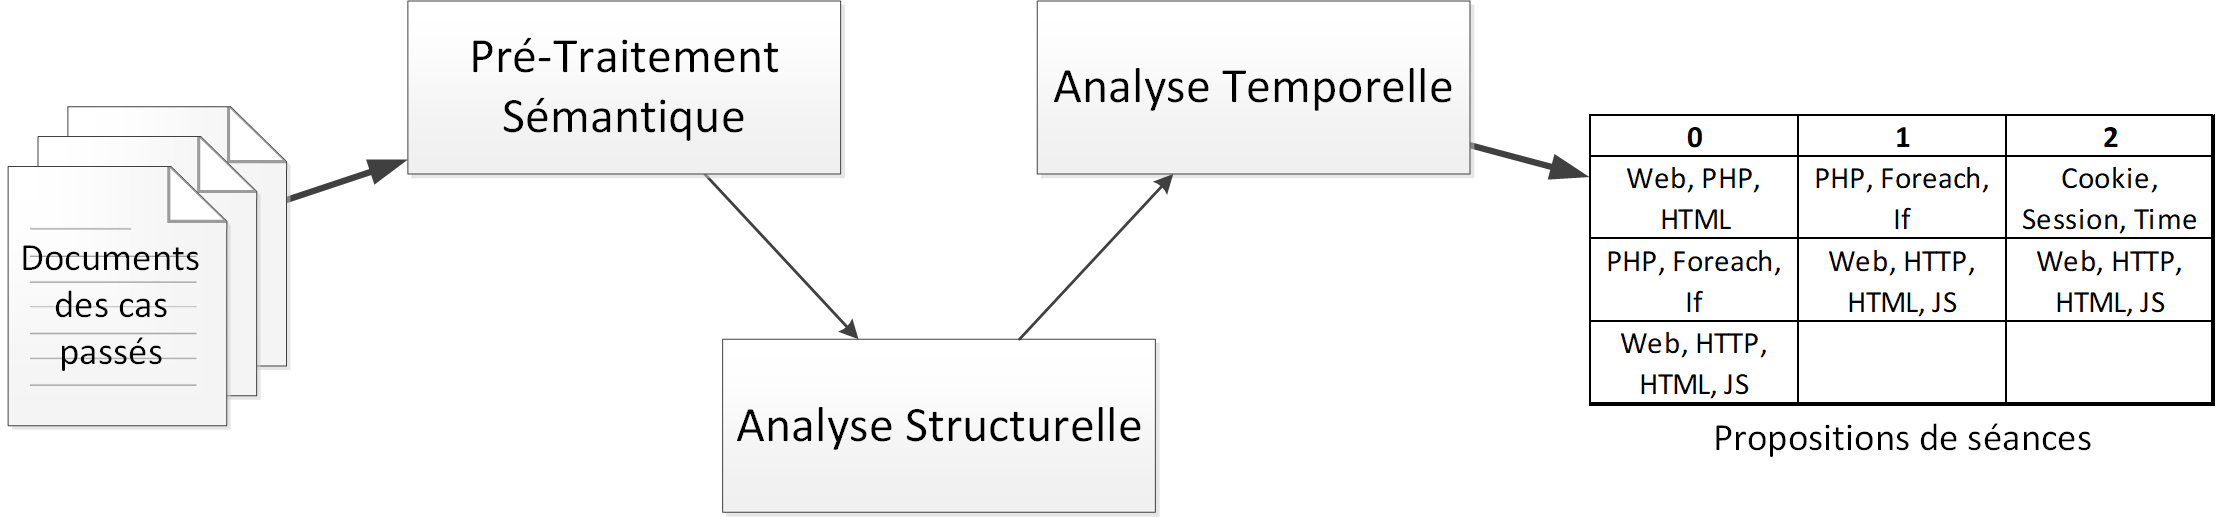
\includegraphics[scale=0.6]{5-Conclusion/images/schema_general+temporel_ESCALIER.png}
}
\caption{La méthode CREA étendue avec l'analyse temporelle}
\label{figure:5-MethodeGenerale+Temporel}
\end{figure}


\bigskip


\begin{figure}[ht]
\centering
\centerline{  % FORCE FIGURE OUTSIDE THE MARGIN !!! BUT STILL CENTERING !!!
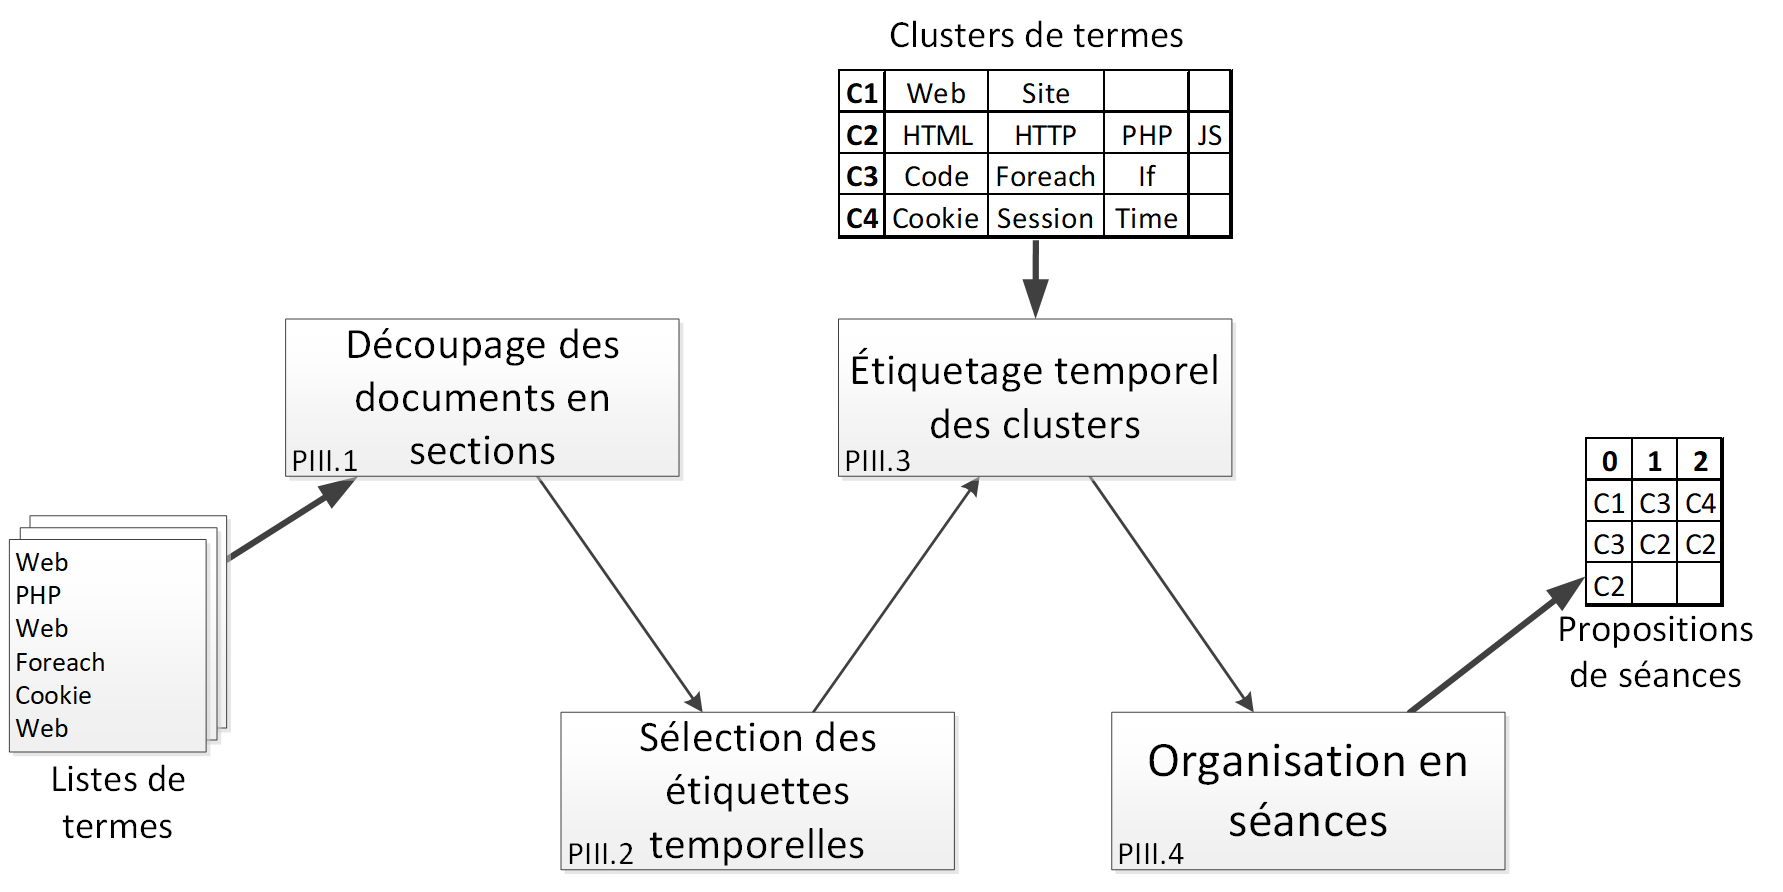
\includegraphics[scale=0.7]{5-Conclusion/images/schema_analyse_temporelle_ESCALIER_2.png}
}
\caption{Les étapes de la phase d'analyse temporelle}
\label{figure:5-III-AnalyseTemporelle}
\end{figure}

\vfill
\hspace{0pt}

\newpage

\subsubsection{Découpage des documents en sections (PIII.1)}
\label{subsubsection:Conclusion:PerspectivesAmeliorations:AnalyseTemporelle:DecoupageDocuments}

Cette étape vise à identifier les proportions de termes par section afin de déduire par la suite quels termes sont spécifiques à certaines sections.
Pour cela, tous les documents sont découpés en autant de sections que de séances exigées par l'utilisateur.
Afin de conserver le meilleur ordonnancement des termes, nous avons décidé d'utiliser les termes issus de l'étape de désambiguïsation (PI.4) décrite en sous-section~\ref{subsection:CREA:PI.4-Desambiguisation}, et non pas du filtrage suivant.
En effet, le filtrage supprimant les termes non pertinents dans l'intégralité de chaque document, la liste de termes est réduite, entraînant une déformation dans la structure des documents.
Bien que les étapes précédents la désambiguïsation suppriment elles aussi des caractères et des mots, la désambiguïsation permet de manipuler des entités reconnues dans des bases de connaissances et donc standardisées dans l'ensemble des documents fournis par l'utilisateur, c'est-à-dire des listes de termes indépendants des problèmes de synonymes et homonymes.

\bigskip

Suite à l'étape de désambiguïsation, une liste de termes reconnus dans des bases de connaissances a été établie.
L'utilisateur indique le nombre de séances qu'il souhaite, et la liste de termes est équitablement divisée en autant de sections.
Le placement des termes dans la structure initiale est ainsi conservée, tout en permettant un découpage selon le nombre de séances visées.
Ce traitement automatique ne nécessite aucune intervention humaine pour corriger ou indiquer où démarre ou finit chaque partie.
Chaque occurrence de terme se voit donc attribuer le numéro de la section associée à sa position dans la liste.
Étant donné que la nature des documents ne permet pas toujours un tel type de découpage, il est nécessaire de ne travailler que sur des documents respectant une organisation séquentielle.
La figure~\ref{figure:5-III-1-Decoupage} illustre le découpage en quatre sections (de 0 à 3) d'un document désambiguïsé sous forme d'une liste de huit termes.


%\begin{figure*} % Figure flottante
\begin{figure}[ht]
\centering
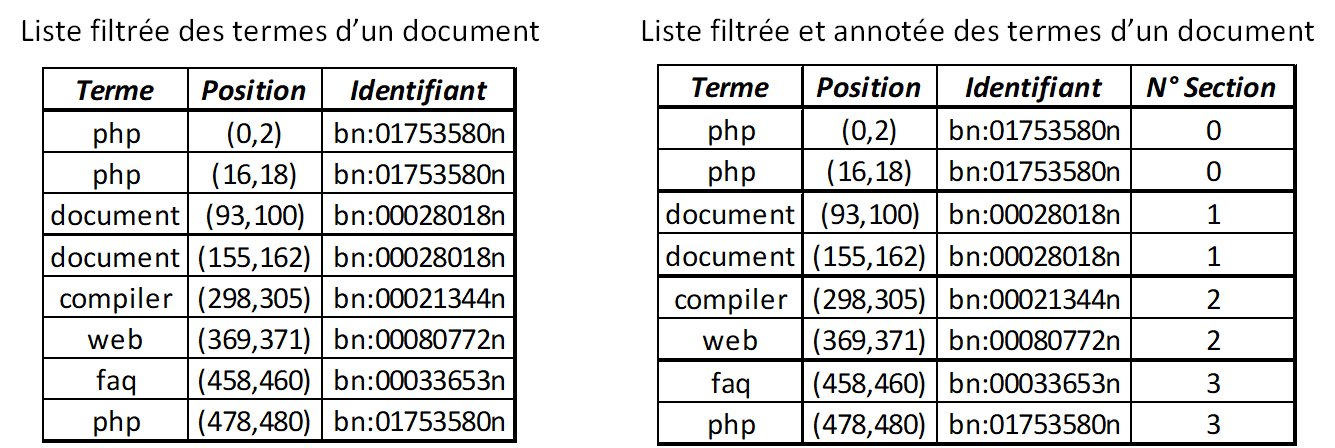
\includegraphics[scale=0.8]{5-Conclusion/images/3-analyse-temporelle/exemple_decoupage_documents.png}
\caption{Découpage d'un document en quatre sections}
\label{figure:5-III-1-Decoupage}
\end{figure}
%\end{figure*} % Figure flottante
% To use it : fig~\ref{label}

\bigskip

Une fois les termes d'un document associés à une section, une proportion de présence de chaque terme dans chaque section est calculée.
Cette proportion permet de connaître la distribution des termes dans chacune des sections d'un document, ce qui contribue à extraire le positionnement des termes les plus importants de l'ensemble des documents.
Le calcul de la proportion des termes dans un document s'effectue comme indiqué dans l'équation~\eqref{equation:5-III-1-Calcul-Proportion-Termes}.

\begin{equation}
\text{\textit{proportion}}(T, P) = \frac{\sum \text{ \textit{des occurrences du terme T dans la section S}}}{\sum \text{ \textit{des occurrences du terme T dans toutes les sections}}} \times 100
\label{equation:5-III-1-Calcul-Proportion-Termes}
\end{equation}


\medskip

La figure~\ref{figure:5-III-1-ProportionDocuments} illustre les deux transformations successives de la liste filtrée et annotée de termes.
Tout d'abord, les proportions d'occurrences des termes dans chaque section sont calculées : \textit{php} apparait \textit{2} fois dans la section \textit{0} sur un total de \textit{3} occurrences, ce qui donne une proportion d'occurrences de \textit{66\%} dans cette section, puis, \textit{php} apparait \textit{1} fois dans la section \textit{3} sur un total de \textit{3} occurrences, ce qui donne une proportion d'occurrences de \textit{33\%} dans cette section.
Les proportions par termes et sections sont ensuite réunies en un seul tableau indiquant les proportions de termes dans chacune des sections.
Le terme \textit{compiler} apparait uniquement en section \textit{2} (\textit{100\%} en \textit{\% S2}) avec \textit{1} seule occurrence, tandis que \textit{php} se trouve à \textit{66\%} en section \textit{0} et \textit{33\%} en section \textit{3} avec un total de \textit{3} occurrences.

\bigskip

On obtient ainsi un tableau récapitulant les termes apparaissant dans chaque document, ainsi que plusieurs autres informations.
Le nombre total d'occurrences de chaque terme et la proportion d'occurrences dans chaque section sont explicités.
Ce tableau permet de voir immédiatement les termes les plus utilisés dans un document, ainsi que leur distribution parmi les sections visées.

\hspace{0pt}
\vfill

\begin{figure}[ht]
\centering
\centerline{  % FORCE FIGURE OUTSIDE THE MARGIN !!! BUT STILL CENTERING !!!
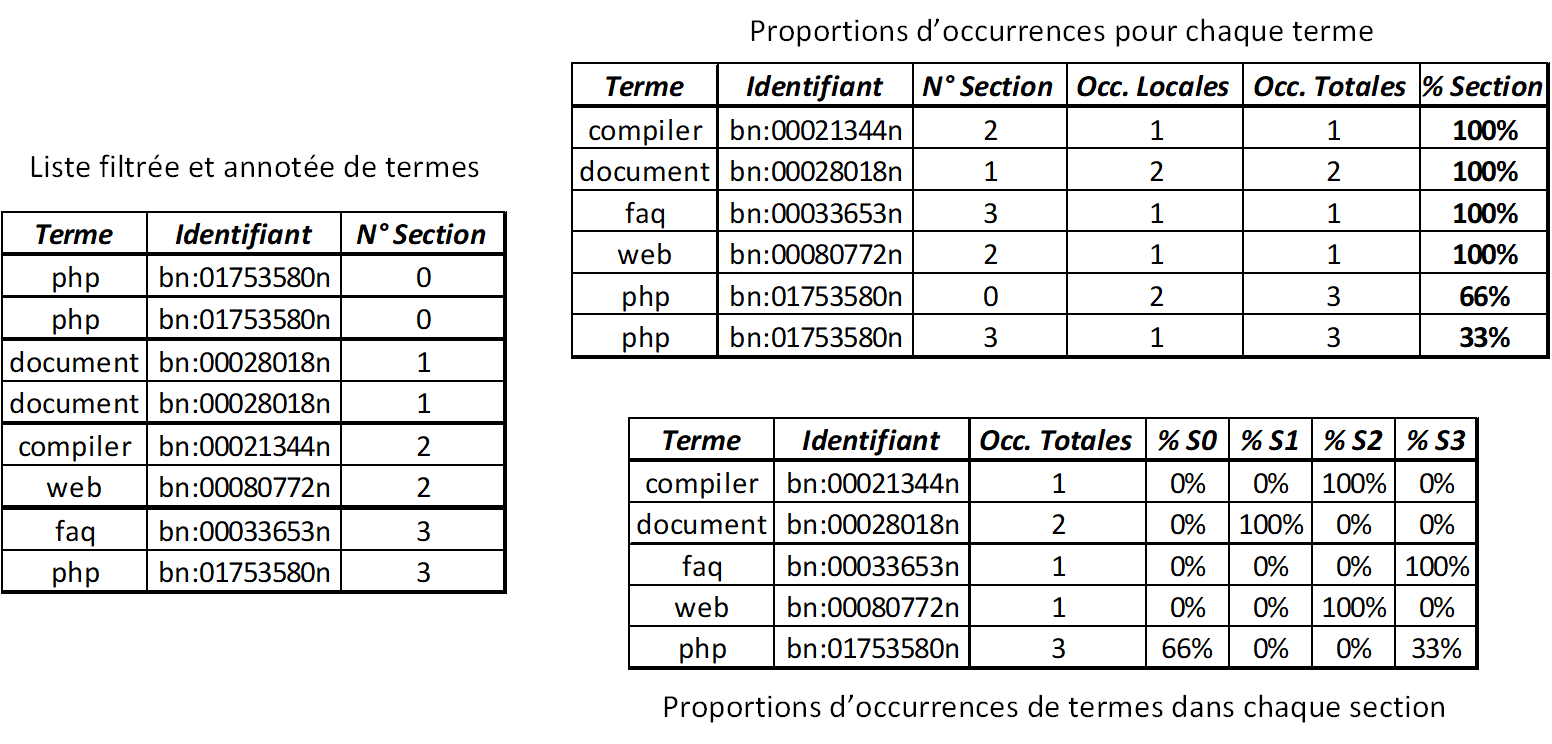
\includegraphics[scale=0.8]{5-Conclusion/images/3-analyse-temporelle/exemple_proportion_documents.png}
}
\caption{Proportion de terme dans chacune des quatre sections du document}
\label{figure:5-III-1-ProportionDocuments}
\end{figure}

\vfill
\hspace{0pt}

\newpage

\subsubsection{Sélection des étiquettes temporelles (PIII.2)}
\label{subsubsection:Conclusion:PerspectivesAmeliorations:AnalyseTemporelle:SelectionEtiquettesTemporelles}

Les tableaux de proportions d'occurrences de termes dans chacun des documents sont fusionnés pour pouvoir obtenir une liste de termes dits \textit{significatifs}.
Les \textit{termes significatifs} correspondent à des termes dont la fréquence d'apparition est supérieure à un seuil (détaillé par la suite) dans les mêmes sections de l'ensemble des documents.
Ces termes sont donc suffisamment fréquents pour être importants et suffisamment concentrés dans quelques sections précises pour qu'il s'agisse de termes spécifiques à ces sections.
Les \textit{termes significatifs} permettent de déterminer les sections dans lesquelles certains termes pourraient être fixés, afin d'organiser temporellement les clusters contenant ces termes.

\bigskip

Les proportions sont analysées afin de mesurer la dispersion des termes dans l'ensemble des sections du document.
Pour cela, le \textit{coefficient de Gini}~\cite{gini1921measurement} est utilisé :
\og \textit{L'indice (ou coefficient) de Gini est un indicateur synthétique permettant de rendre compte du niveau d'inégalité pour une variable et sur une population donnée. Il varie entre 0 (égalité parfaite) et 1 (inégalité extrême). Entre 0 et 1, l'inégalité est d'autant plus forte que l'indice de Gini est élevé} \fg~\cite{coeffginiinsee}.
En effet, pour comprendre si un terme est dispersé de façon égale dans toutes les sections, ou au contraire si celui-ci est concentré dans une ou quelques sections seulement, le coefficient de Gini est parfaitement adapté.

\paragraph{Explications du coefficient de Gini :}
Le coefficient de Gini d'une distribution correspond au double de l'aire issue de la différence entre la droite représentant une distribution parfaitement équitable (une diagonale) et la courbe de Lorenz de la distribution étudiée (formée par la somme successive des valeurs de la distribution)~\cite{mussard2006decomposition}.
Le graphique~\ref{figure:5-III-2-ExempleCourbeLorenz} montre la distribution $ 5, 10, 40, 5, 40 $ réordonnée en $ 5, 5, 10, 40, 40 $ pour former une courbe de Lorenz (courbe bleue) passant sous la droite de la distribution équitable (droite rouge).
Il existe plusieurs manières de calculer le coefficient de Gini~\cite{mornet2014decomposition}.
Une de ces manières utilise l'équation de Kendal et Stuart~\eqref{equation:5-III-2-Coefficient-Gini-Kendal-1963} où $ n $ correspond au nombre d'éléments dans la distribution, et $ y_{1} , y_{2} , ... , y_{n} $ correspond à chaque élément de la distribution~\cite{kendall1963advanced}\cite{pyatt1976interpretation}.
La formule~\eqref{equation:5-III-2-Coefficient-Gini-Mookherjee-1982} issue de l'approche de Mookherjee et Shorrocks~\cite{mookherjee1982decomposition} étant plus simple à implémenter, celle-ci est retenue.
Elle s'appuie sur la moyenne de la distribution ($ \mu $) ainsi que sur la somme des différences absolues des éléments de la distribution divisée par le carré du nombre d'éléments.
Pour obtenir le coefficient de Gini, on divise la moyenne des différences absolues des éléments entre eux ($ Moyenne ( | y_{1} - y_{1} | , | y_{1} - y_{2} | , ... , | y_{n} - y_{n} | ) $) par la moyenne des éléments ($ Moyenne ( y_{1}, y_{2}, ..., y_{n} ) $), puis diviser le tout par $ 2 $.


\medskip

\begin{equation}
G = \frac{ (1 / 2 n^{2}) \, \overset{n}{\underset{i = 1}{\sum}} \overset{n}{\underset{j = 1}{\sum}} \, | y_{i} - y_{j} | }{ (1 / n) \, \overset{n}{\underset{i = 1}{\sum}} \, y_{i}}
\label{equation:5-III-2-Coefficient-Gini-Kendal-1963}
\end{equation}

\medskip

\begin{equation}
G = \frac{1}{2 \mu n^{2}} \, \overset{n}{\underset{i = 1}{\sum}} \overset{n}{\underset{j = 1}{\sum}} \, | y_{i} - y_{j} |
\label{equation:5-III-2-Coefficient-Gini-Mookherjee-1982}
\end{equation}

\medskip

\begin{figure}[ht!]
\centering
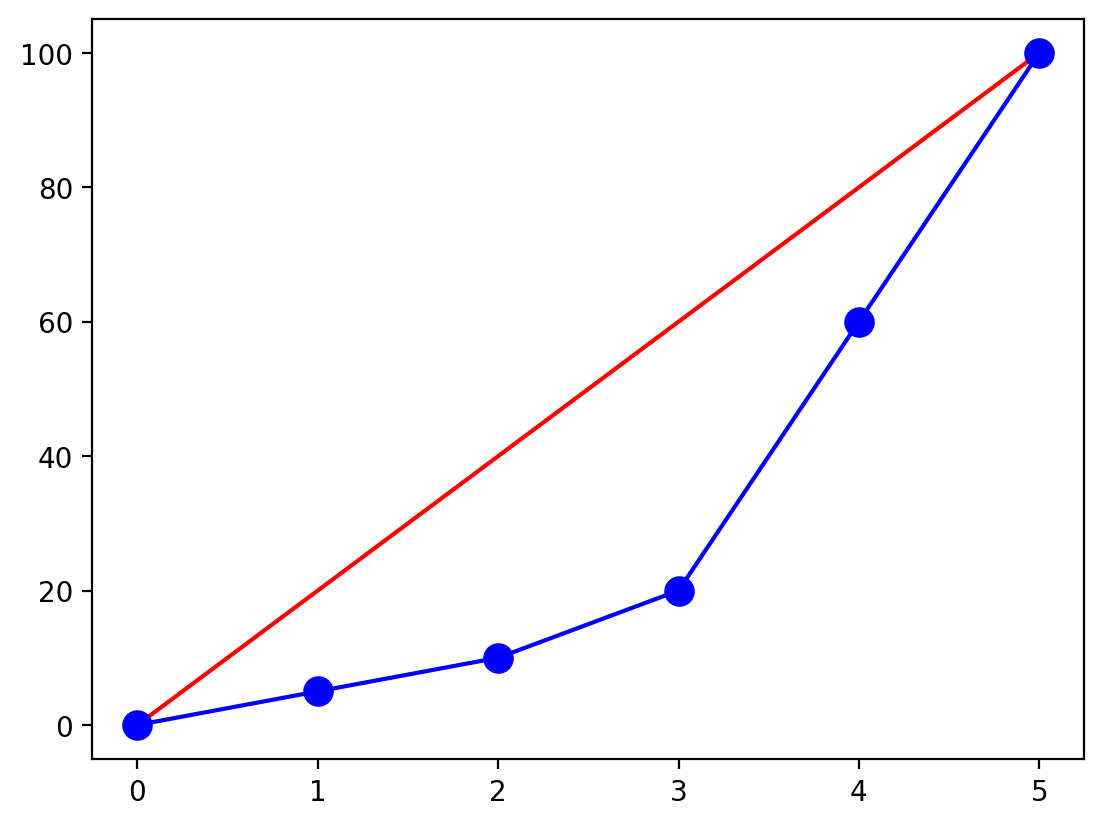
\includegraphics[scale=0.6]{5-Conclusion/images/3-analyse-temporelle/exemple_courbe_lorenz_simple.png}
\caption{Exemple d'une courbe de Lorenz (en bleu) issue de la distribution $ 5, 10, 40, 5, 40 $ }
\label{figure:5-III-2-ExempleCourbeLorenz}
\end{figure}



Pour mesurer le degré de concentration d'un terme dans les différentes sections d'un document, on calcule donc le coefficient de Gini sur les proportions d'occurrences du terme dans chaque section.
Les termes dont le coefficient de Gini est supérieur ou égal à $ 0,3 $ sont considérés comme suffisamment concentrés pour être analysés plus en profondeur.
Chaque proportion d'occurrences des termes conservés est ensuite comparée à la moyenne des proportions d'occurrences du terme considéré.
Seules les proportions strictement supérieures à la moyenne sont considérées comme significatives.
Ces choix empiriques proviennent du fait que le coefficient de Gini calcule un degré de concentration qui varie indépendamment de la moyenne (qui peut rester fixe).
Un coefficient de Gini élevé sur une distribution où quelques valeurs dépassent la moyenne implique nécessairement que les autres valeurs sont beaucoup plus faibles, donc que les valeurs au dessus de la moyenne sont beaucoup plus grandes que les autres valeurs.
À l'inverse, un coefficient de Gini faible implique dans tous les cas que les valeurs sont proches les unes des autres, y compris celles qui dépassent la moyenne.
Nous avons fixé le seuil du coefficient de Gini à $ 0,3 $ pour les besoins de la méthode CREA, car cette valeur sépare correctement les distributions trop peu concentrées des distributions suffisamment concentrées.
La figure~\ref{figure:5-III-2-ExempleCourbeLorenz3Proportions} montre trois exemples de proportions différentes pour cinq sections.
Les histogrammes en jaune indiquent chaque valeur de la distribution, c'est-à-dire la proportion d'occurrences d'un terme dans chaque section (pour rappel, la courbe de Lorenz est formée par l'addition successive de ces valeurs).
La somme des proportions étant toujours égale à $ 100 $, pour un document coupé en cinq sections la moyenne (droite verte en pointillés) sera toujours de $ 20 $.

\medskip

\begin{itemize}
\item La première distribution $ 10, 15, 20, 25, 30 $ donne un coefficient de Gini de $ 0,200 $, ce qui indique que la distribution est plutôt équitable : le terme est présent dans toutes les sections avec une faible différence des occurrences.
\item La deuxième distribution $ 0, 0, 0, 10, 90 $ donne un coefficient de Gini de $ 0,760 $, ce qui indique que la distribution est inéquitable : quelques sections concentrent toutes les occurrences du terme.
\item La dernière distribution $ 5, 5, 10, 40, 40 $ donne un coefficient de Gini de $ 0,424 $, ce qui indique une certaine iniquité entre les parties : le terme est présent dans toutes les sections, mais les occurrences sont plus élevées dans deux d'entre elles.
\end{itemize}
Dans cette dernière distribution, on voit effectivement que les proportions $ 40 \% $ et $ 40 \% $ sont particulièrement plus grandes que les trois autres proportions (respectivement $ 5 \% $, $ 5 \% $, et $ 10 \% $).
Empiriquement parlant, ceci permet d'affirmer qu'un terme se trouve majoritairement dans les deux sections associées à ces proportions.
Le coefficient de Gini étant supérieur à $ 0,3 $ dans deux des trois distributions (représentant un document chacune), on ne sélectionne que les sections dont les proportions (barres jaunes des histogrammes) sont supérieures à la moyenne (droite verte en pointillés).
Ainsi, les termes sont considérés comme \textit{significatifs} aux sections concernées dans les distributions des deux documents.


%\begin{figure*} % Figure flottante
\begin{figure}[ht]
\centering
%\includegraphics[width=3in]{images/VerySmallModels_text.png}
%%\includegraphics[scale=0.6]{images/VerySmallModels_text.png}
\centerline{  % FORCE FIGURE OUTSIDE THE MARGIN !!! BUT STILL CENTERING !!!
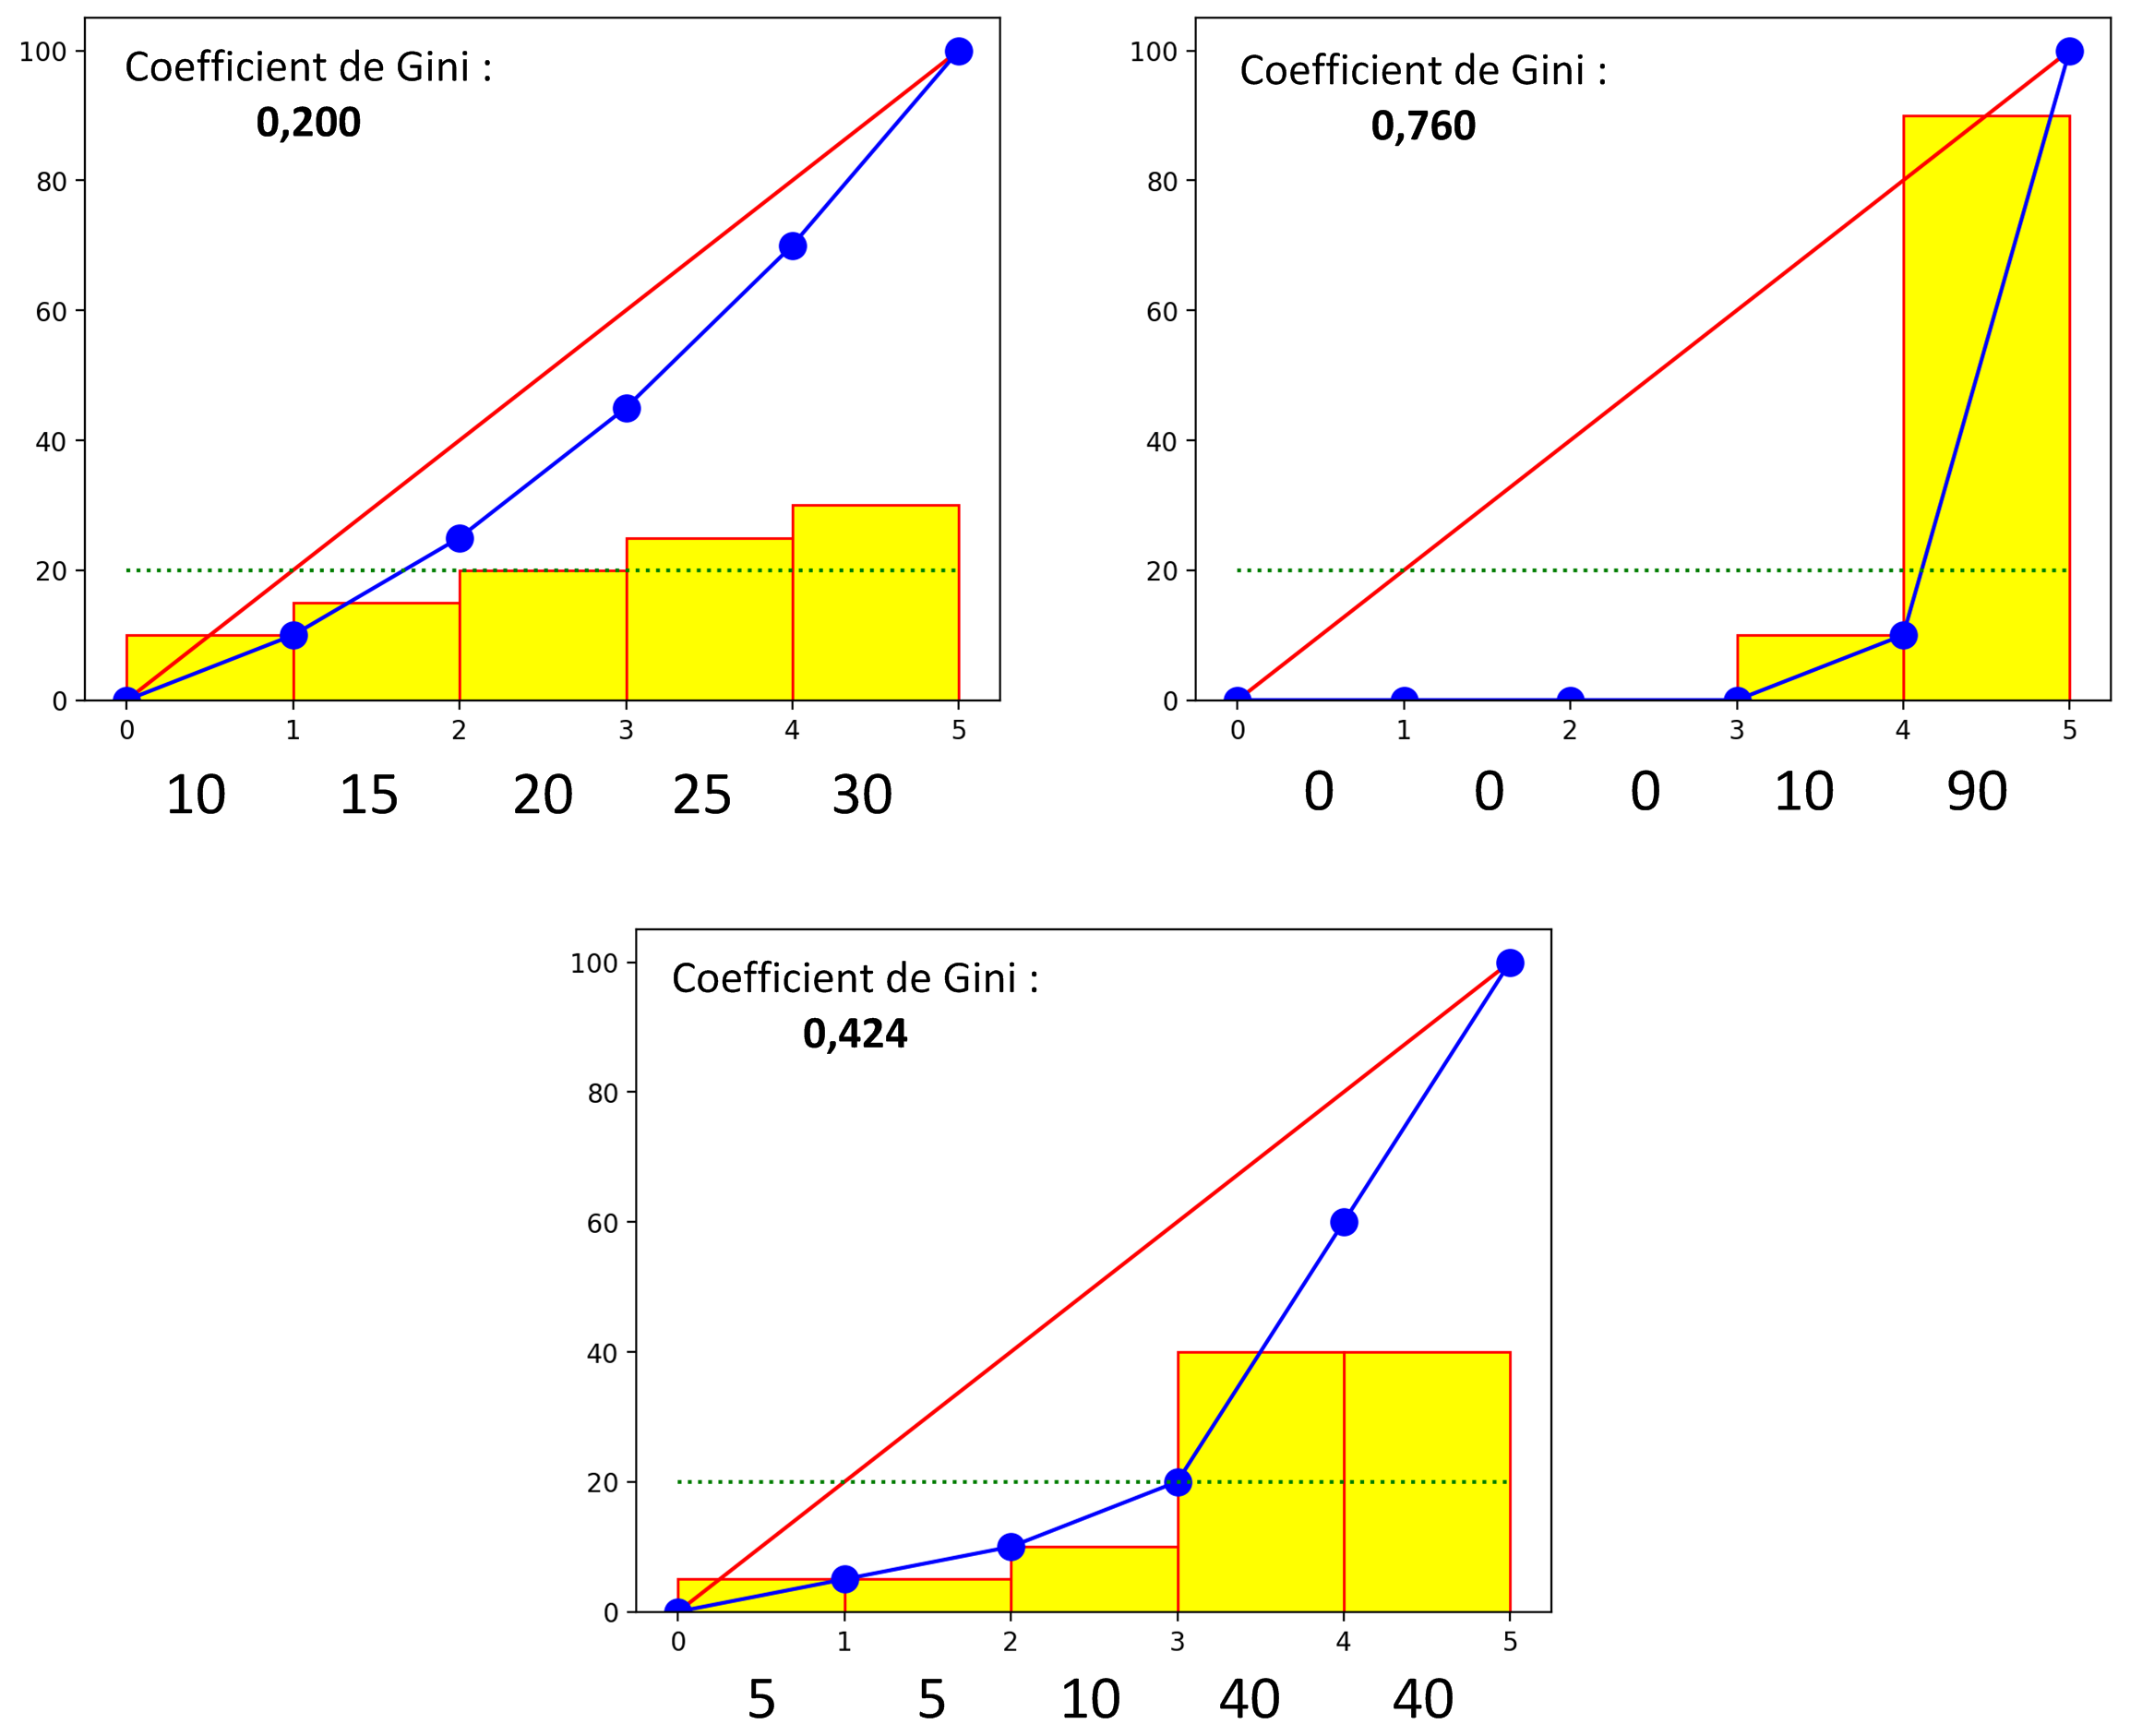
\includegraphics[scale=0.6]{5-Conclusion/images/3-analyse-temporelle/exemple_courbes_lorenz.png}
}
\caption{Trois exemples de proportions différentes sur cinq sections}
\label{figure:5-III-2-ExempleCourbeLorenz3Proportions}
\end{figure}
%\end{figure*} % Figure flottante
% To use it : fig~\ref{label}


Afin de considérer les termes comme \textit{significatifs}, la forte concentration de chaque terme par partie par document ($ G > 0,3 $) n'est pas suffisante.
Une moyenne des occurrences de l'ensemble des termes est calculée, et seuls les termes dont les occurrences sont supérieures à la moyenne sont considérés pour la suite des traitements.
Ainsi, les termes suffisamment présents dans le document et suffisamment concentrés dans certaines sections sont considérés comme des \textit{termes significatifs}.
Ce test est formalisé par la formule~\eqref{equation:5-III-2-Test-Termes-Significatif}, où $ T $ correspond à un terme parmi l'ensemble de ceux du document (de $ 1 $ à $ n $), et $ G $ correspond au coefficient de Gini.

\medskip

%Est\_Significatif(x) = (Occurrences(Termes(x)) > \frac{ \overset{n}{\underset{i = 1}{\sum}} {Occurrences(Termes(i))} }{n}) \and (G(Termes(x)) > 0,3)
\begin{equation}
\text{\textit{EstSignificatif}}(T_{x}) = (\text{\textit{Occurrences}}(T_{x}) > \frac{1}{n} \overset{n}{\underset{i = 1}{\sum}} {\text{\textit{Occurrences}}(T_{i})})    \wedge     (G(T_{x}) > 0,3)
\label{equation:5-III-2-Test-Termes-Significatif}
\end{equation}

\medskip

La figure~\ref{figure:5-III-2-ExempleTermesSignificatifs} illustre un exemple pas à pas du calcul des termes significatifs, et des sections auxquelles ils sont associés, pour un document coupé en quatre sections avec cinq termes.
\begin{enumerate}
\item Les proportions d'occurrences des termes dans chaque sections sont agrégées dans un unique tableau.
\item Le coefficient de Gini est calculé pour chaque terme.
Le document étant coupé en quatre sections, la moyenne des proportions est donc de $ 25\% $.
Seules les proportions supérieures à $ 25\% $ associées à un terme dont le coefficient de Gini est supérieur à $ 0,3 $ sont conservées (avec un $ 1 $).
\item La moyennes des occurrences de l'ensemble des termes est calculée pour déterminer quels termes sont fréquents ou non.
Seuls les termes dont la valeur d'occurrences est supérieure à la moyenne seront conservés.
\item La liste finale des termes significatifs est produite : la colonne \textit{significatif} indique avec un $ 1 $ que le terme est fortement concentré dans une ou quelques sections~(indiquée(s) dans les colonnes \textit{S0}, \textit{S1}, \textit{S2}, et/ou \textit{S3}).
\end{enumerate}
Dans cet exemple, on peut voir que les termes \textit{compiler} et \textit{document} sont concentrés dans certaines sections mais trop peu présents dans l'ensemble du document pour être retenus.
Le terme \textit{web} n'est pas assez concentré dans certaines sections pour être retenu.
À l'inverse, les termes \textit{faq} et \textit{php} sont concentrés dans deux sections précises chacun (S0, S1, et S2) et suffisamment fréquents (au delà de la moyenne d'occurrences) pour être considérés comme significatifs dans ces sections pour ce document.

\bigskip

Ces traitements permettent d'obtenir pour chaque document une liste de termes significatifs dans chacune des sections.
Afin d'ordonner par la suite les fragments réutilisables et former des scénarios plus concrets, une agrégation des termes significatifs de l'ensemble des documents est réalisée.
Les termes sont reconnus par leur identifiant unique, puis sont agrégés selon les sections et documents dans lesquels ils sont considérés comme significatifs.
Le tableau généré permet de connaître pour chaque terme dans quel(s) document(s) et section(s) il est considéré comme significatif.
La figure~\ref{figure:5-III-2-ExempleTableauTermesSignificatifs} illustre comment les termes significatifs de trois documents sont rassemblés en un tableau.
On peut voir que le terme \og \textit{size} \fg identifié par \og \textit{$bn{:}00016413n$} \fg est significatif pour la section \textit{S2} dans le document \textit{C3}, mais aussi pour la section \textit{S3} dans les documents \textit{C2} et \textit{C3}.
Cette organisation liant les termes, les documents, et les numéros de sections, se combine facilement aux clusters de termes précédemment créés : il devient possible d'ajouter une information temporelle dans les clusters, grâce aux numéros de sections associées aux termes et documents.


\newpage

\hspace{0pt}
\vfill

\begin{figure}[ht]
\centering
%%% 0.8
\centerline{  % FORCE FIGURE OUTSIDE THE MARGIN !!! BUT STILL CENTERING !!!
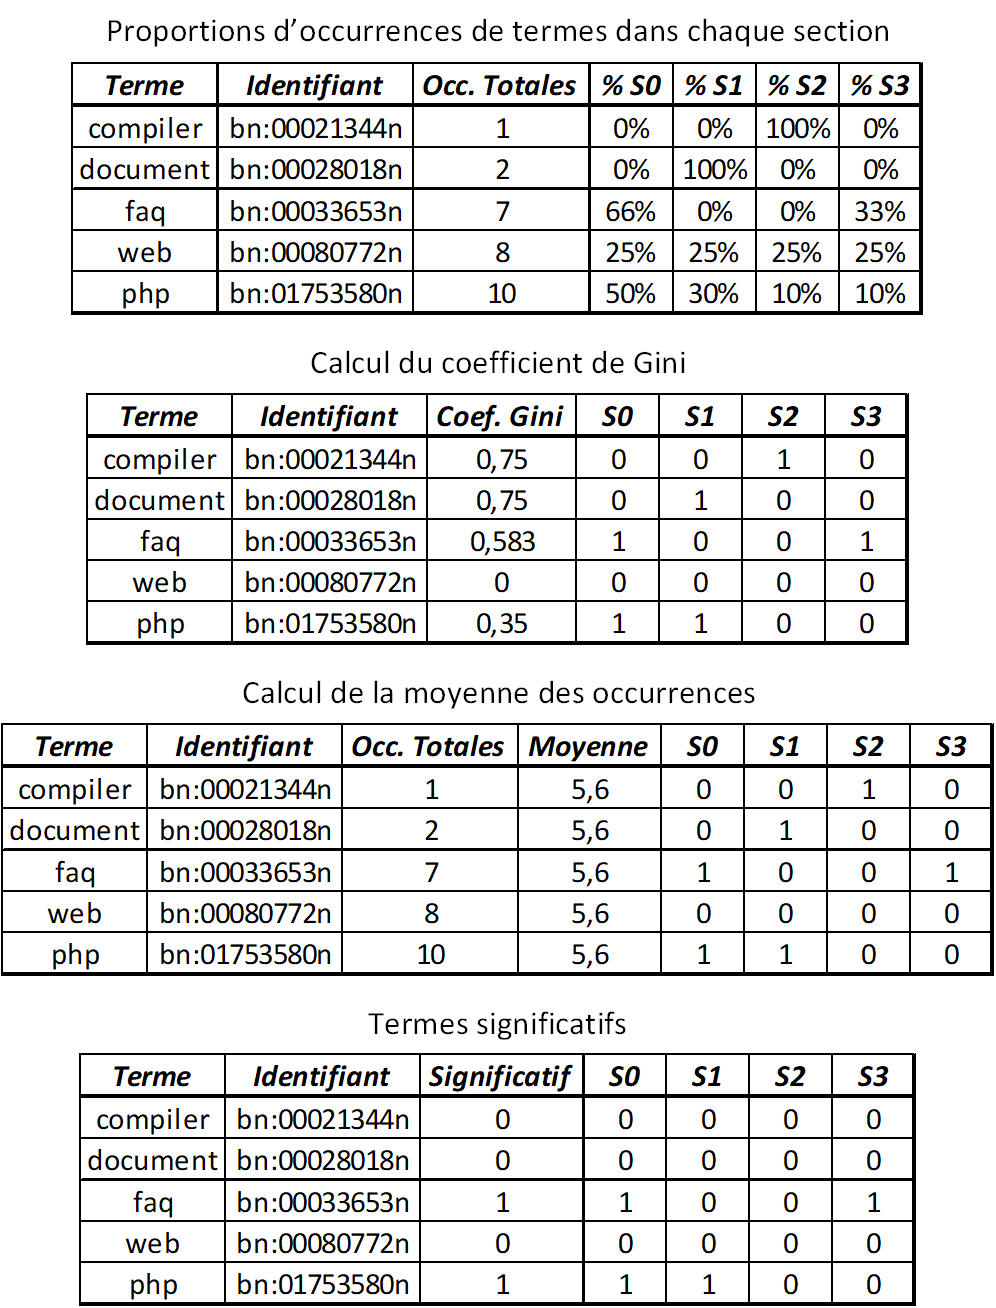
\includegraphics[scale=1]{5-Conclusion/images/3-analyse-temporelle/exemple_termes_significatifs.png}
}
\caption{Exemple de calcul des termes significatifs d'un document}
\label{figure:5-III-2-ExempleTermesSignificatifs}
\end{figure}

\vfill
\hspace{0pt}

\newpage

\hspace{0pt}
\vfill

\begin{figure}[ht]
\centering
\centerline{  % FORCE FIGURE OUTSIDE THE MARGIN !!! BUT STILL CENTERING !!!
%%% 0.8
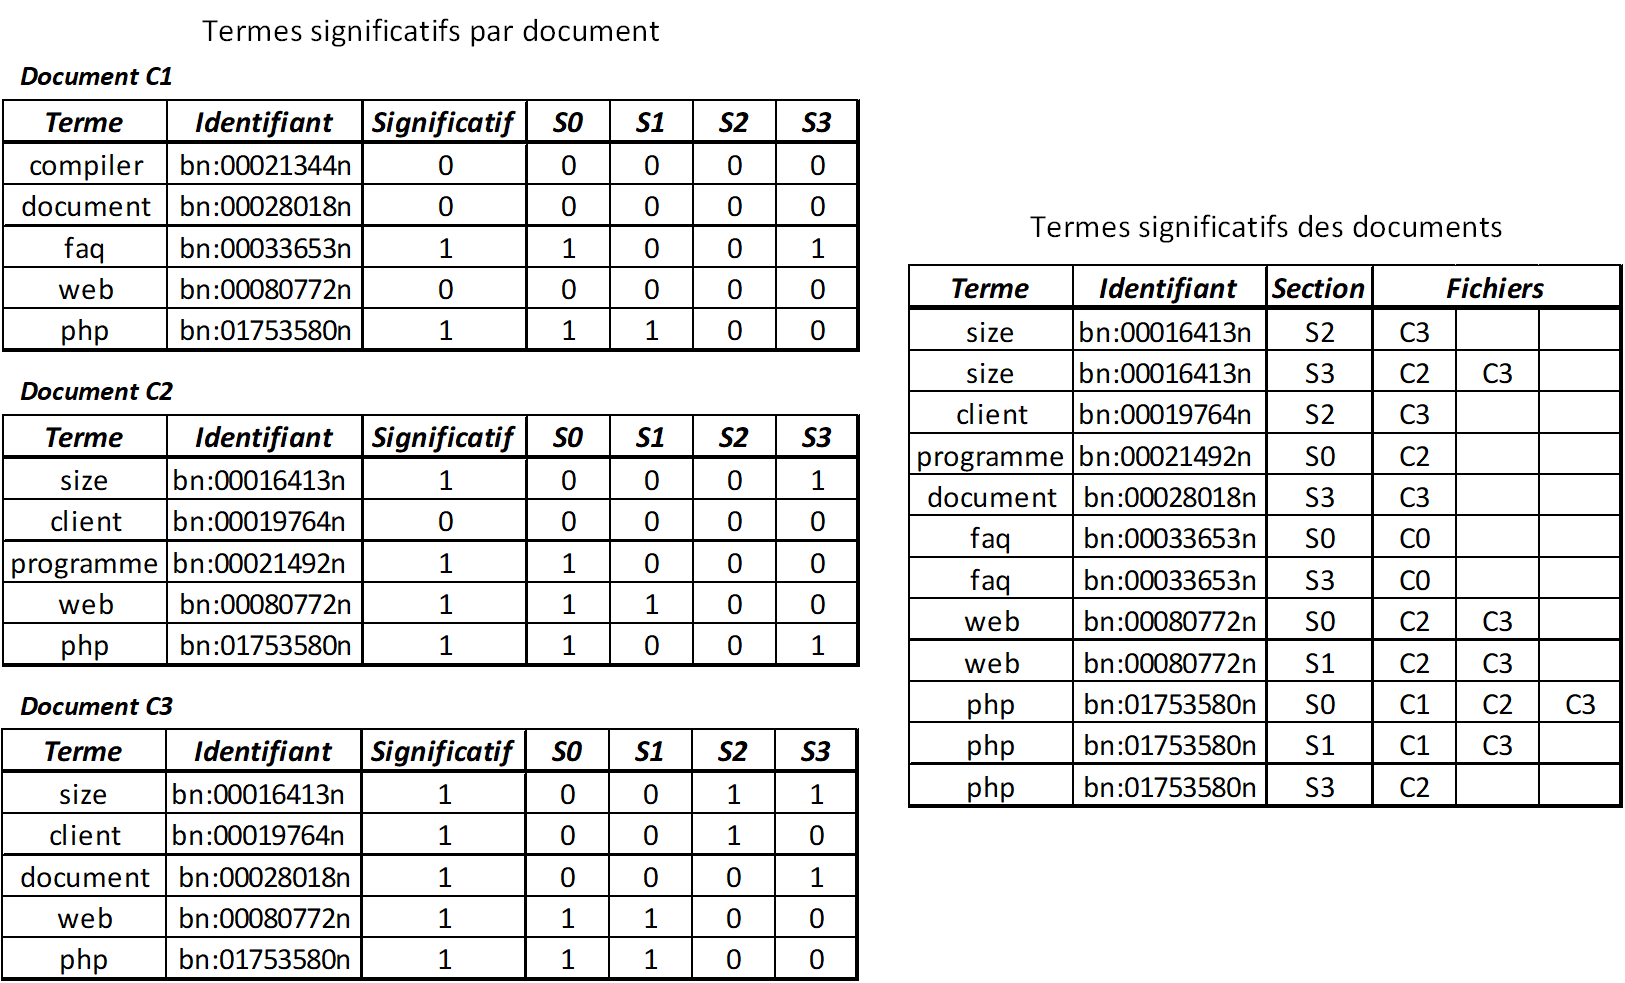
\includegraphics[scale=0.85]{5-Conclusion/images/3-analyse-temporelle/exemple_tableau_termes_significatifs.png}
}
\caption{Exemple d'agrégation des termes significatifs de chaque document en un tableau}
\label{figure:5-III-2-ExempleTableauTermesSignificatifs}
\end{figure}

\vfill
\hspace{0pt}

\newpage

\subsubsection{Étiquetage temporel des clusters (PIII.3)}
\label{subsubsection:Conclusion:PerspectivesAmeliorations:AnalyseTemporelle:EtiquetageTemporelClusters}

Les clusters de termes précédemment formés, représentant des fragments réutilisables pour former une structure, peuvent maintenant être enrichis d'une information temporelle, ordonnancés.
Cette étape vise à fusionner les clusters de termes avec l'information temporelle embarquée par les termes, pour pouvoir étiqueter temporellement les clusters et proposer un ordonnancement.

\bigskip

Nous avons tout d'abord testé le simple ajout des numéros de sections associées à chaque terme, de sorte à effectuer une \textit{union} de toutes les sections proposées par les termes d'un même cluster.
Cette \textit{union} était cependant trop ambiguë dans nos essais, car quasiment tous les clusters étaient étiquetés d'à peu près toutes les sections.
Puis, nous avons testé l'équivalent d'une \textit{intersection} des sections proposées par les termes significatifs d'un même cluster (seuls les termes disposant d'une information temporelle sont pris en compte).
Cette \textit{intersection} était trop restrictive et n'étiquetait que les clusters contenant le moins de termes significatifs, engendrant des clusters peu voire pas du tout pertinents pour l'ordonnancement temporel.
Finalement, nous avons préféré un \textit{vote à la majorité} des sections des termes significatifs.

\bigskip

Les termes significatifs (i.e., ceux disposant d'une information temporelle) \og votent \fg pour chacune de leurs sections.
Chaque terme donne un point (\og vote \fg pour) à chaque section dans laquelle il est considéré comme terme significatif.
Les sections retenues sont celles disposant strictement de plus de la moitié des votes dans chacun des clusters.
La figure~\ref{figure:5-III-3-ExempleFusionClustersTermesSignificatifs} illustre ce vote à la majorité dans le cas d'un cours sur quatre séances (donc quatre clusters et quatre sections).
Le terme significatif \textit{liste} est étiqueté des quatre sections auxquelles il est rattaché \textit{S0}, \textit{S1}, \textit{S2}, et \textit{S3}.
Le terme significatif \textit{foreach} est étiqueté des deux sections auxquelles il est rattaché \textit{S2} et \textit{S3}.
Les autres termes significatifs sont étiquetés eux aussi.
Le cluster 1 contient \textit{5} termes significatifs, c'est-à-dire qu'une section sera retenue si elle obtient strictement plus de $ 5 \div 2 = 2,5 $ voix, donc en pratique au moins \textit{3} voix.
Le consensus se fait donc sur les sections \textit{S0}, \textit{S2}, et \textit{S3}.
La section \textit{S1} ne disposant que de 2 voix, elle n'est pas retenue.
Le cluster 4 contient \textit{4} termes significatifs, c'est-à-dire qu'une section sera retenue si elle obtient strictement plus de $ 4 \div 2 = 2 $ voix, donc en pratique au moins \textit{3} voix.
Chaque section n'obtenant que 2 voix, aucune n'est retenue, et le cluster n'est pas étiqueté temporellement.
À l'issue de cette étape, les clusters qui le peuvent sont étiquetés temporellement.

\newpage

\hspace{0pt}
\vfill

\begin{figure}[ht!]
\centering
\centerline{  % FORCE FIGURE OUTSIDE THE MARGIN !!! BUT STILL CENTERING !!!
%%% 0.8
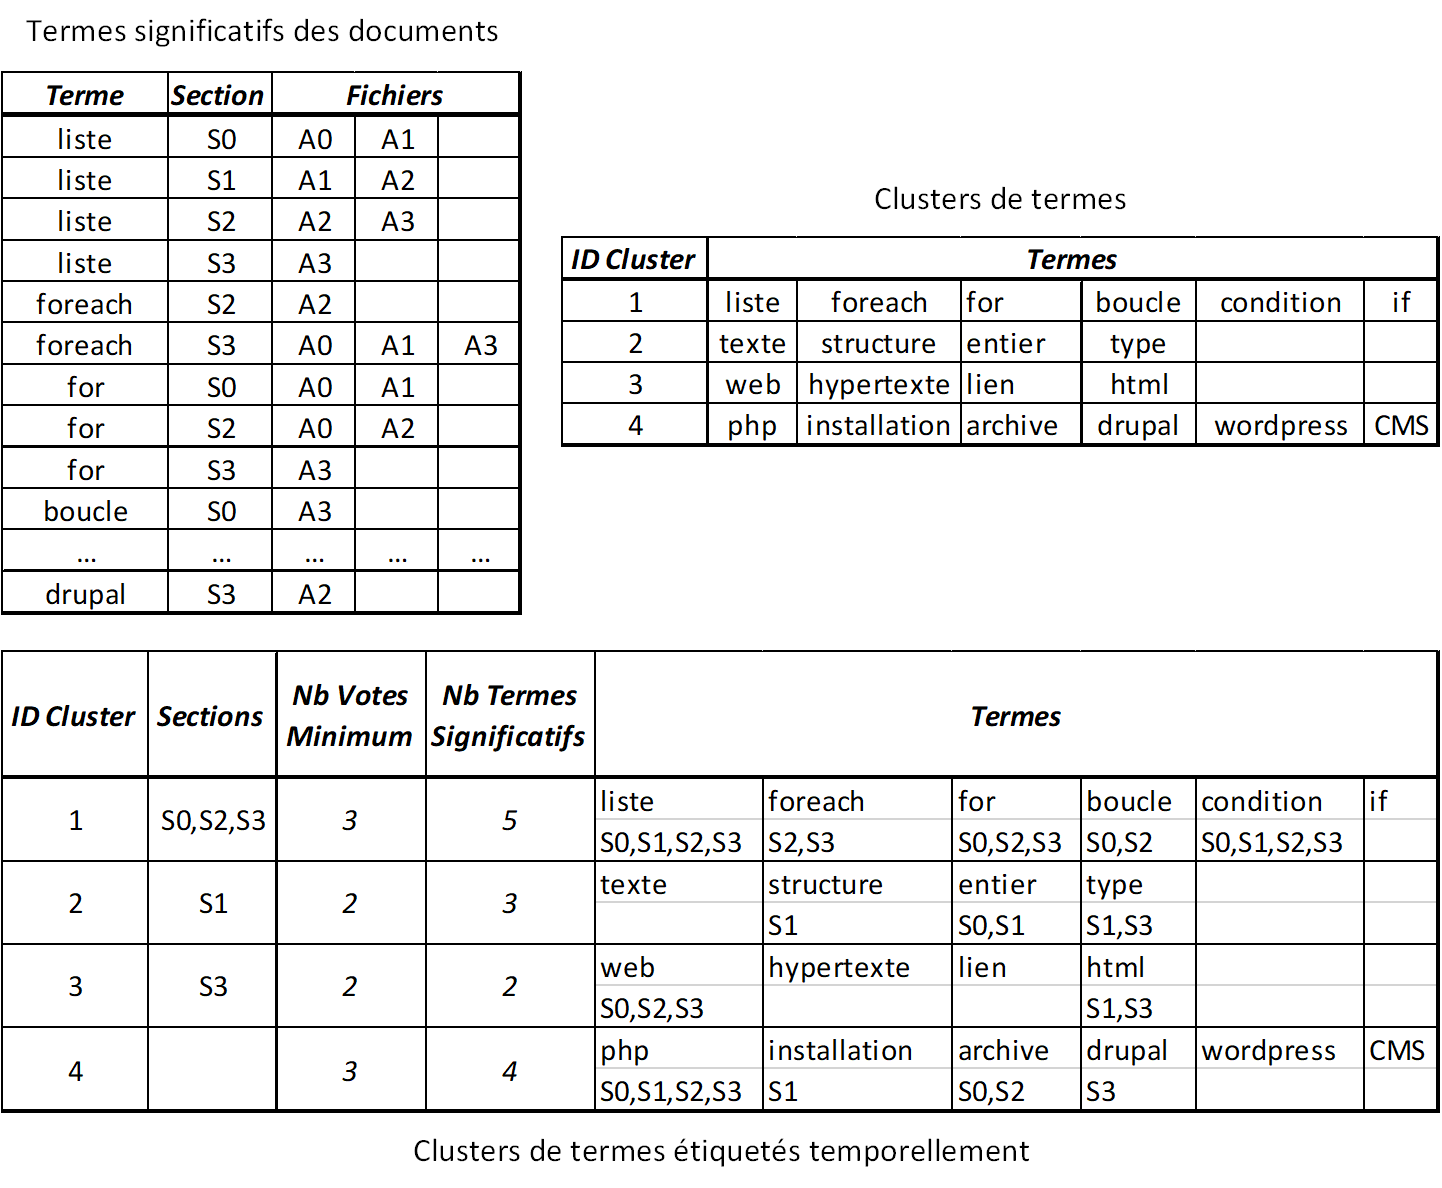
\includegraphics[scale=1]{5-Conclusion/images/3-analyse-temporelle/exemple_fusion_clusters_termes_significatifs.png}
}
\caption{Exemple d'étiquetage des clusters avec un vote strictement supérieur à la majorité absolue}
\label{figure:5-III-3-ExempleFusionClustersTermesSignificatifs}
\end{figure}

\vfill
\hspace{0pt}

\newpage

\subsubsection{Organisation en séances (PIII.4)}
\label{subsubsection:Conclusion:PerspectivesAmeliorations:AnalyseTemporelle:OrganisationSeances}

Les clusters étiquetés temporellement disposent d'une information sur leurs possibles placements dans le nouveau cas.
Afin de proposer des scénarios possibles constitués de séances et des notions étudiées dans chacune, un changement de point de vue est nécessaire.
Cette étape vise à passer du point de vue des clusters, vers celui des séances, pour permettre à l'utilisateur de visualiser les organisations possibles des séances et choisir celle qui lui convient.

\bigskip

L'utilisateur ayant précédemment indiqué le nombre de séances souhaitées, les clusters sont analysés pour ordonner ceux-ci.
Pour chaque numéro de séance, les clusters disposant de l'étiquette temporelle associée au même numéro de section sont proposés en premier, puis, ceux ne disposant d'aucune information temporelle sont ensuite proposés.
L'utilisateur dispose ainsi d'une vue globale de l'ensemble des séances à venir.
Celui-ci est ainsi guidé et peut choisir quels clusters conserver ou retirer au fur et à mesure de l'exécution de son cas, ou précisément dans le contexte de l'enseignement, de son cours.
La figure~\ref{figure:5-III-4-ExempleOrganisationSeances} illustre un exemple de réorganisation dans le cas de cours en quatre séances (donc quatre clusters et quatres sections réorganisés en quatre séances).
Le cluster 4 n'étant pas étiqueté, il est proposé en dernier choix lors de toutes les séances.
Le cluster 1 étant étiqueté aux sections \textit{S0}, \textit{S2}, et \textit{S3}, il est proposé lors des séances 0, 2 et 3.

\bigskip

Une fois l'organisation en séances réalisée, l'enseignant dispose d'une vue globale d'un déroulé possible de cours par rapport à l'ensemble des supports sélectionnés en entrée et au nombre de séances demandées.
Cette organisation des séances se calcule donc automatiquement d'un point de vue utilisateur, considérant nos différents réglages et choix empiriques sur l'ensemble de la chaîne de traitements.

\newpage

\hspace{0pt}
\vfill

\begin{figure}[ht]
\centering
\centerline{  % FORCE FIGURE OUTSIDE THE MARGIN !!! BUT STILL CENTERING !!!
%%% 0.8
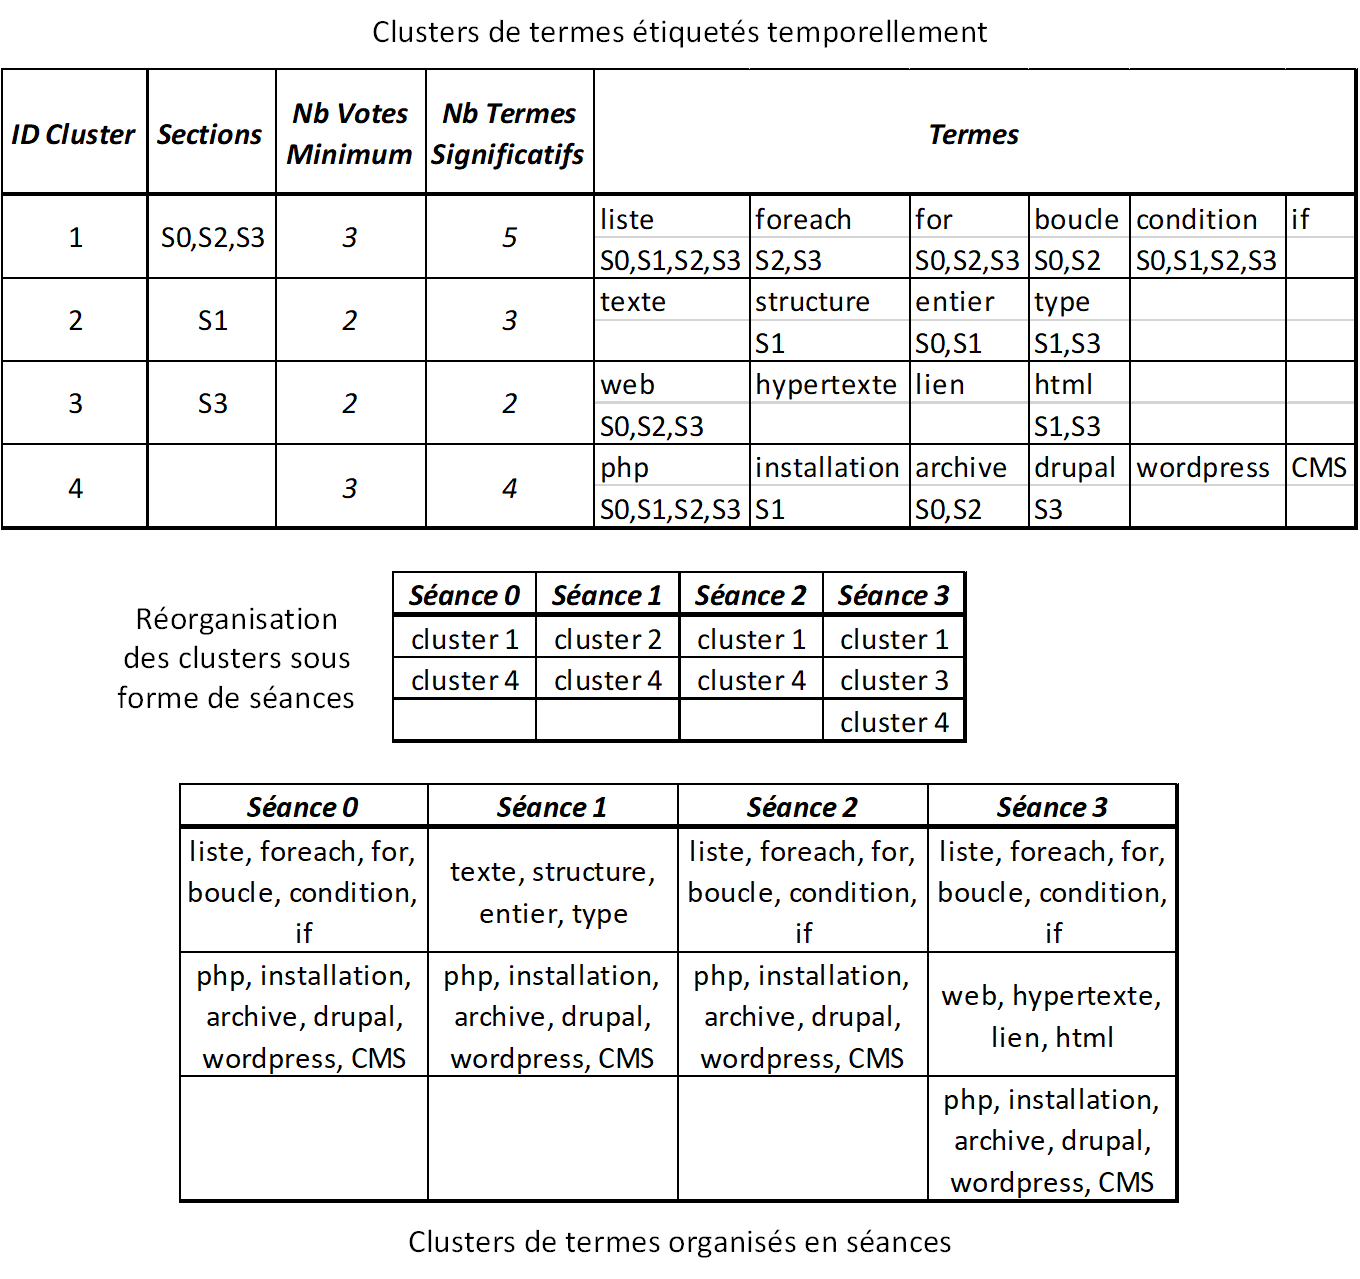
\includegraphics[scale=1]{5-Conclusion/images/3-analyse-temporelle/exemple_organisation_seances.png}
}
\caption{Exemple d'organisation en séances}
\label{figure:5-III-4-ExempleOrganisationSeances}
\end{figure}

\vfill
\hspace{0pt}

\newpage

\subsubsection{Résultats préliminaires et discussion}
\label{subsubsection:Conclusion:PerspectivesAmeliorations:AnalyseTemporelle:EvaluationDiscussion}

Nous avons succinctement évalué cette extension et présentons maintenant quelques résultats partiels.
Seul le scénario n°1 de référence vu en section~\ref{subsection:Evaluation:ProtocoleEvaluation:ScenariosEvaluation} a été testé.
Pour rappel, ce cas visait à construire un cours de développement web avec PHP sur 8 séances à partir de 9 supports existants, dont 3 au format texte long et 6 au format diapositives.
Les résultats de l'étiquetage temporel des clusters (PIII.3) sont tout d'abord présentés sur la figure~\ref{figure:5-Experience-EtiquetageClusters}.
Puis, les résultats de l'organisation sous forme de séances (PIII.4) sont présentés sur la figure~\ref{figure:5-Experience-SeancesOrganisees}.


\hspace{0pt}
\vfill


\begin{figure}[ht!]
\centering
\centerline{  % FORCE FIGURE OUTSIDE THE MARGIN !!! BUT STILL CENTERING !!!
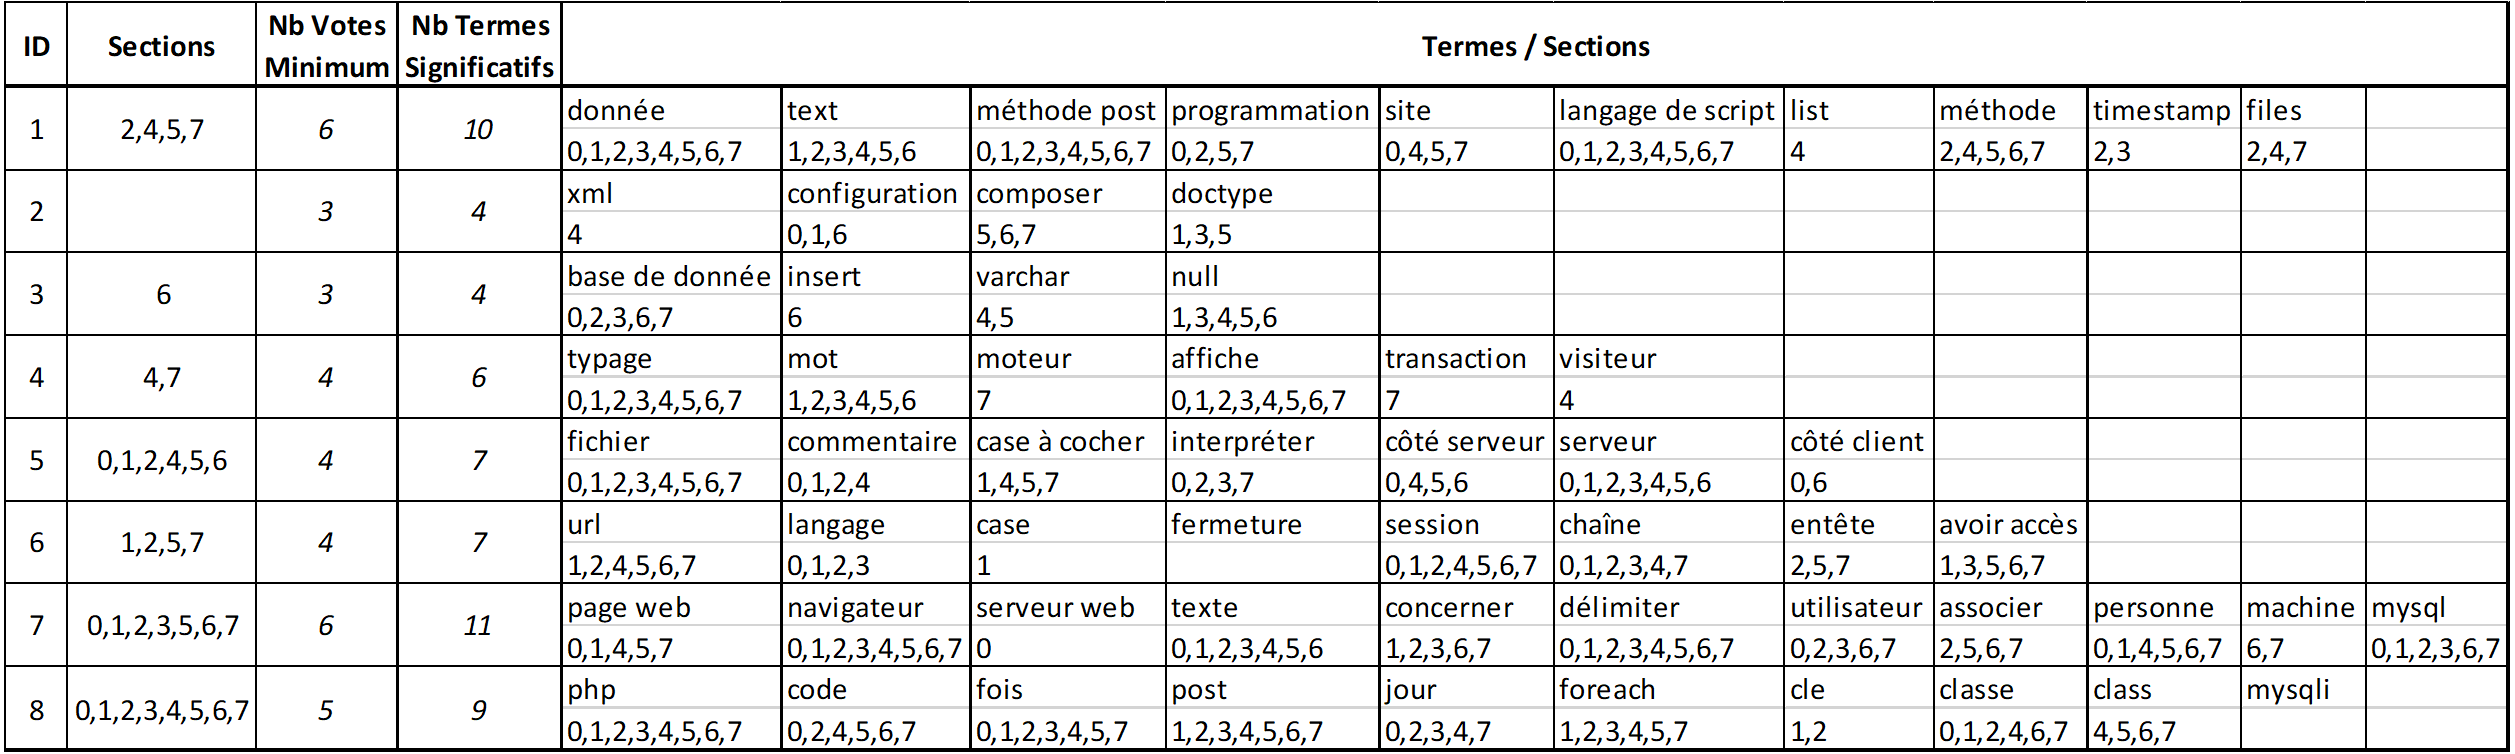
\includegraphics[scale=0.6]{5-Conclusion/images/exemples/clusters-S=H-B=1.00-votants.png}
}
\caption{Résultats de l'étiquetage temporel des clusters (PIII.3) du cas n°1 référence}
\label{figure:5-Experience-EtiquetageClusters}
\end{figure}



\begin{figure}[ht!]
\centering
\centerline{  % FORCE FIGURE OUTSIDE THE MARGIN !!! BUT STILL CENTERING !!!
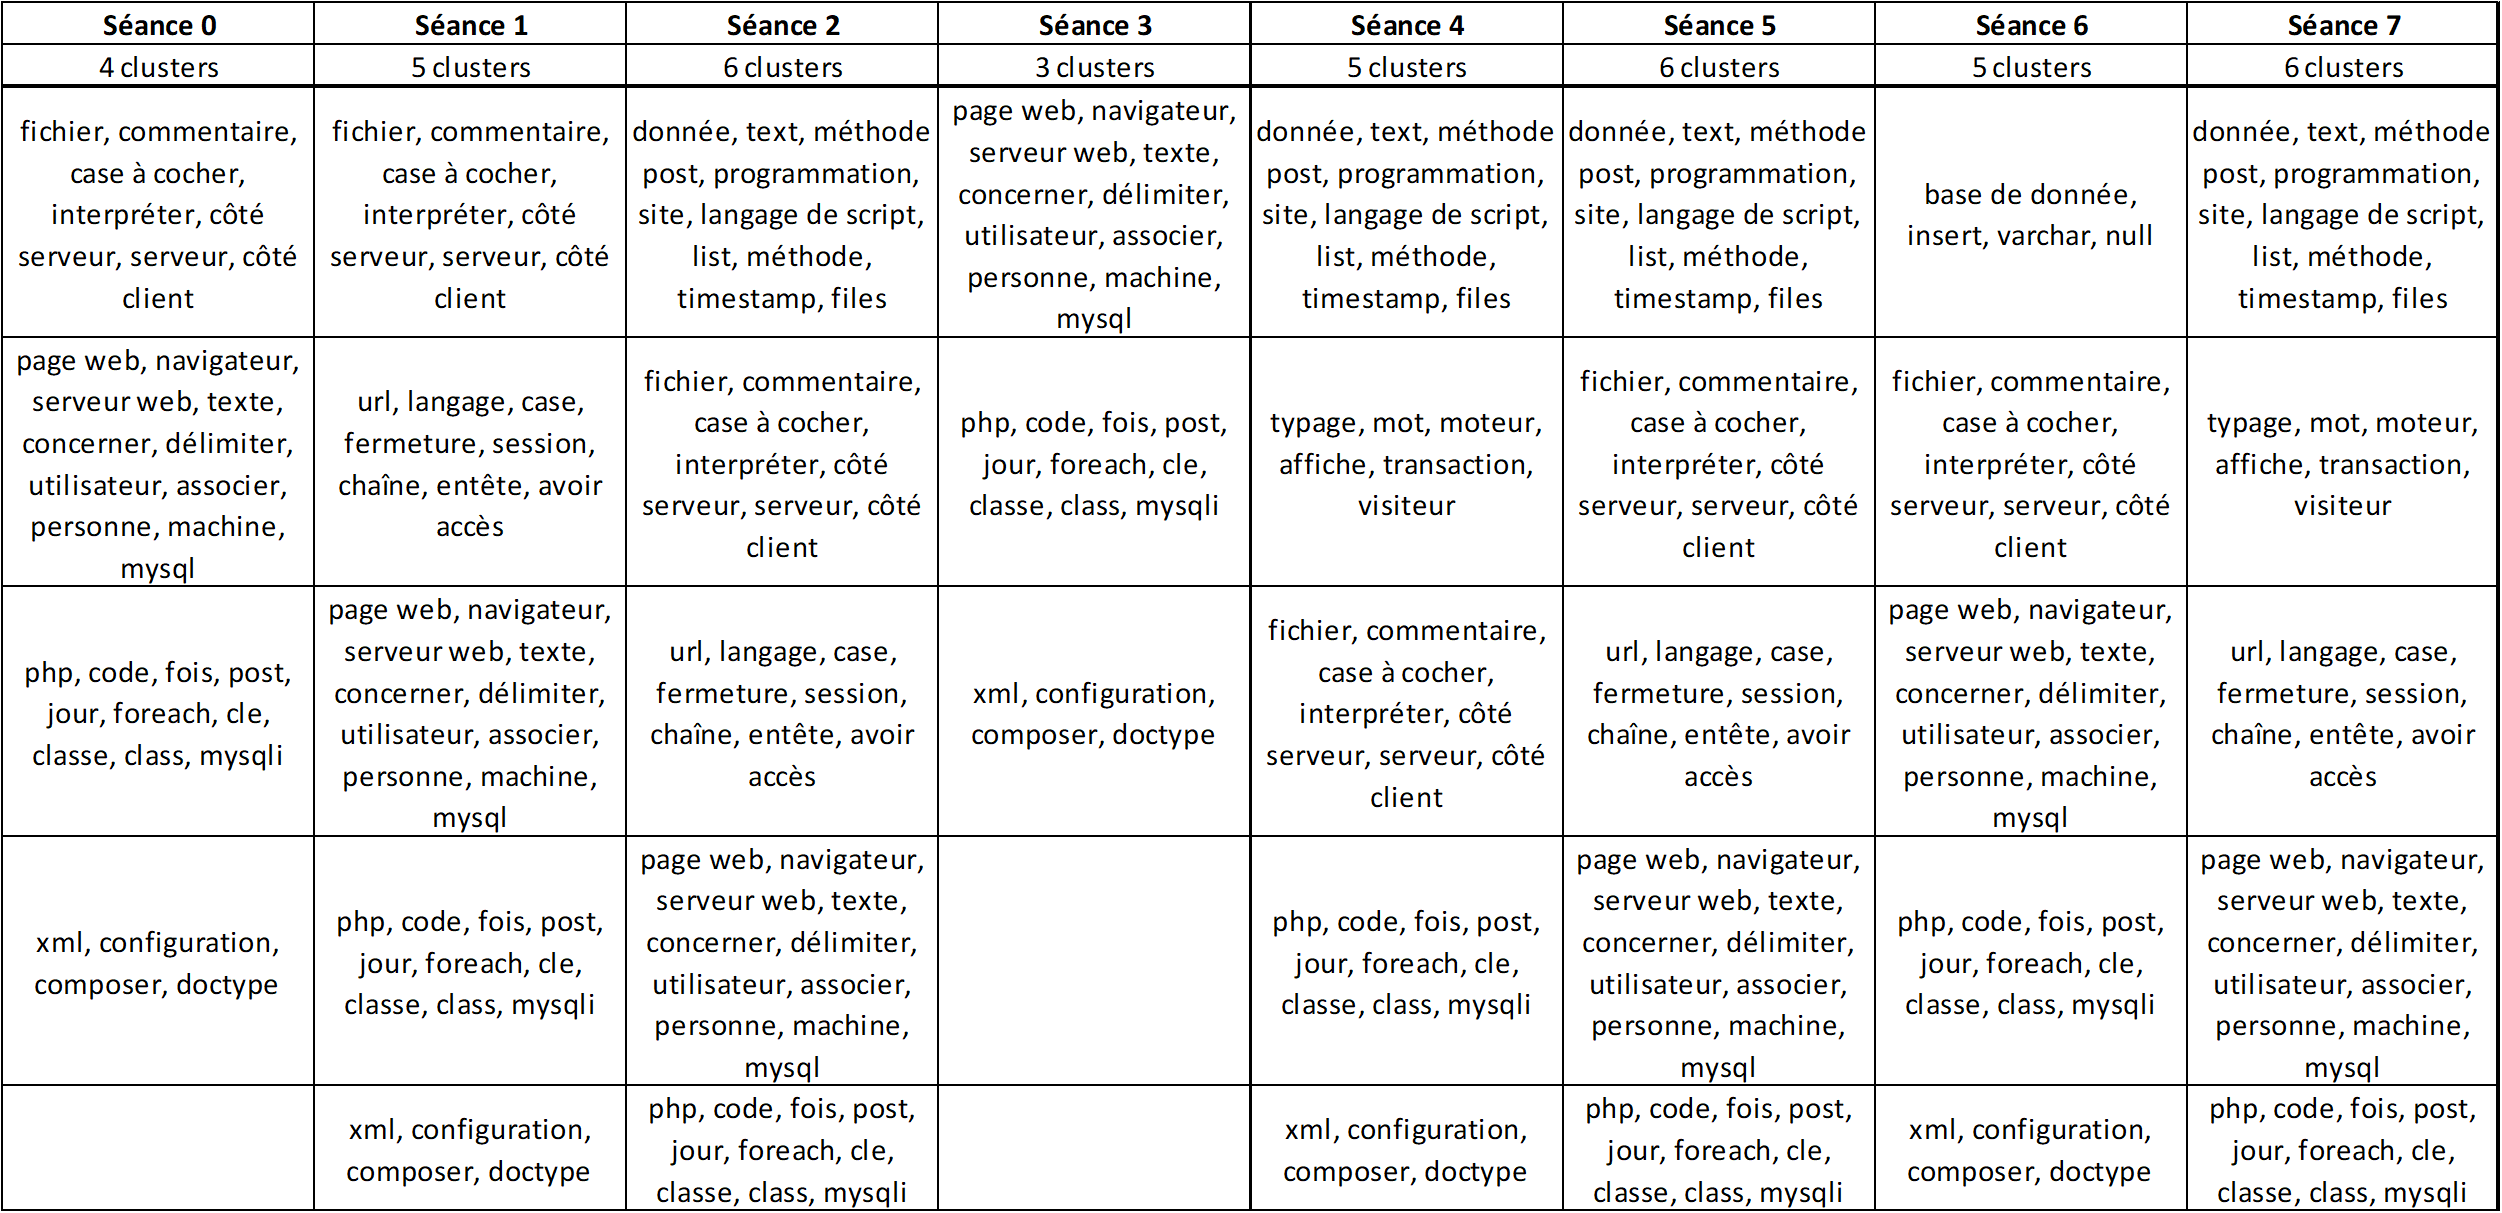
\includegraphics[scale=0.6]{5-Conclusion/images/exemples/scenario-S=H-B=1.00.png}
}
\caption{Résultats de l'organisation en séances (PIII.4) du cas n°1 référence}
\label{figure:5-Experience-SeancesOrganisees}
\end{figure}


\vfill
\hspace{0pt}


\newpage

Une première analyse de l'étiquetage temporel des clusters sur la figure~\ref{figure:5-Experience-EtiquetageClusters} nous permet de constater tout d'abord qu'un seul des 8 clusters n'est pas étiqueté ($ 13\% $), 2 clusters sont étiquetés avec une ou deux sections ($ 25\% $), 2 clusters sont étiquetés avec quatre sections ($ 25\% $), et 3 clusters sont étiquetés avec six sections ou plus ($ 38\% $).
Cela signifie que 4 clusters ($ 50\% $) peuvent quasiment être placés sur n'importe quelle séance.
Parmi les 4 autres clusters, 2 peuvent être placés dans la moitié des séances ($ 25\% $).
Seuls 2 clusters sont explicitement placés dans une ou deux séances ($ 25\% $).
Les résultats montrent qu'il est difficile de fixer automatiquement les clusters sur quelques séances précises avec la méthode actuelle.
L'étiquetage tel quel donne des propositions d'organisation à l'utilisateur qui reste seul décideur.

\bigskip

Cependant, un résultat encourageant montre que le cluster n°3 contenant les termes \og \textit{base de données, insert, varchar, null} \fg semble explicitement placé en séance 6, c'est-à-dire à l'avant dernière séance.
Ce cluster rassemble des termes qui sont tous apparentés au thème de la base de données.
Les 3 cours au format texte l'abordent au moins au milieu, 2 d'entre eux en parlent en plus entre le début et le milieu, et 1 présente à la fin de nombreux projets utilisant parfois de la base de données.
Concernant les 6 cours au format diapositives, 1 cours n'aborde pas ce thème, 4 cours l'abordent vers la fin, et 1 mentionne très succinctement quelques termes de ce thème à la fin.
De manière générale, 6 cours en parlent au moins un peu à la fin ($ 67\% $), 3 en parlent au milieu ($ 33\% $), 2 en parlent vers le début ($ 22\% $), et 1 ne l'aborde pas du tout ($ 11\% $).
D'un point de vue purement statistique, ce thème peut être proposé prioritairement vers la fin.
Étant donné le faible nombre de tests, il peut aussi s'agir d'un cas extrême ou de bruit, qui normalement ne serait pas pris en compte.

\bigskip

Cette difficulté à placer les clusters limite l'exploitation telle quelle des résultats par un utilisateur.
Nous proposons trois solutions pour résoudre ce problème :
\begin{itemize}
\item Une première solution de contournement serait de ne présenter à l'utilisateur qu'une seule séance à la fois, depuis la première jusqu'à la dernière, afin qu'il choisisse lui-même quel cluster présenter à chacune des séances sans être submergé d'un excès d'information.
\item Une autre solution pourrait être de revoir la sélection des étiquettes temporelles : un meilleur algorithme de vote pourrait améliorer les résultats (au lieu de l'\textit{union}, \textit{intersection}, ou \textit{vote} des sections).
\item Une dernière solution serait de mieux extraire les étiquettes temporelles : le découpage actuel étant très simple, il pourrait être envisagé d'extraire la structure des supports en analysant le sommaire ou les titres uniquement, mais cela implique un travail très poussé lors de la phase de reconnaissance optique (PI.2), donc avant la désambiguïsation (PI.3) et sa standardisation des termes.
\end{itemize}

\bigskip

Nous présentons cependant quelques opportunités offertes par cette organisation temporelle.
L'analyse temporelle actuelle est spécialisée sur les documents organisés de façon séquentielle.
Dans le cadre de l'enseignement supérieur et de la recherche, les articles de recherche ne sont pas du tout organisés de la même manière qu'un support de cours : il est déconseillé d'appliquer la phase d'analyse temporelle actuelle sur des articles.
Cependant, il est tout de même actuellement possible de construire des clusters avec des documents de nature variée, puis, de rechercher l'ordonnancement temporel uniquement à partir des documents organisés séquentiellement.

\bigskip

Nous avons vu que la méthode exige des documents dont le contenu principal est du texte, sous-entendu que de nombreux autres médias existent, afin de construire des clusters de termes.
En posant l'hypothèse qu'il est possible d'adapter la phase d'analyse temporelle selon la nature de l'organisation temporelle des documents, on pourrait extraire un ordonnancement temporel depuis tous les types de documents organisés.
Là où les supports de cours classiques sont séquentiels, les articles de recherche respectent eux aussi certaines règles selon les domaines (par exemple : introduction, revue de la littérature, contribution(s), expérience(s), discussion(s), conclusion).
Des techniques de détection de rupture appliquées aux textes permettent typiquement d'effectuer un découpage thématique et chronologique~\cite{boufaden2002decoupage}\cite{fallery2007quatre}.
Ainsi, il devient possible d'extraire les termes des introduction et contributions de plusieurs articles sur une durée donnée d'une même équipe de recherche, afin de voir l'évolution des projets et/ou les voies approfondies pour en déduire quels termes étaient porteurs à différentes époques.
Cette dimension temporelle est donc particulièrement attrayante sur les possibilités qu'elle offre.


\newpage

\hspace{0pt}
\vfill

%\begin{figure*} % Figure flottante
\begin{figure}[ht!]
\centering
\centerline{  % FORCE FIGURE OUTSIDE THE MARGIN !!! BUT STILL CENTERING !!!
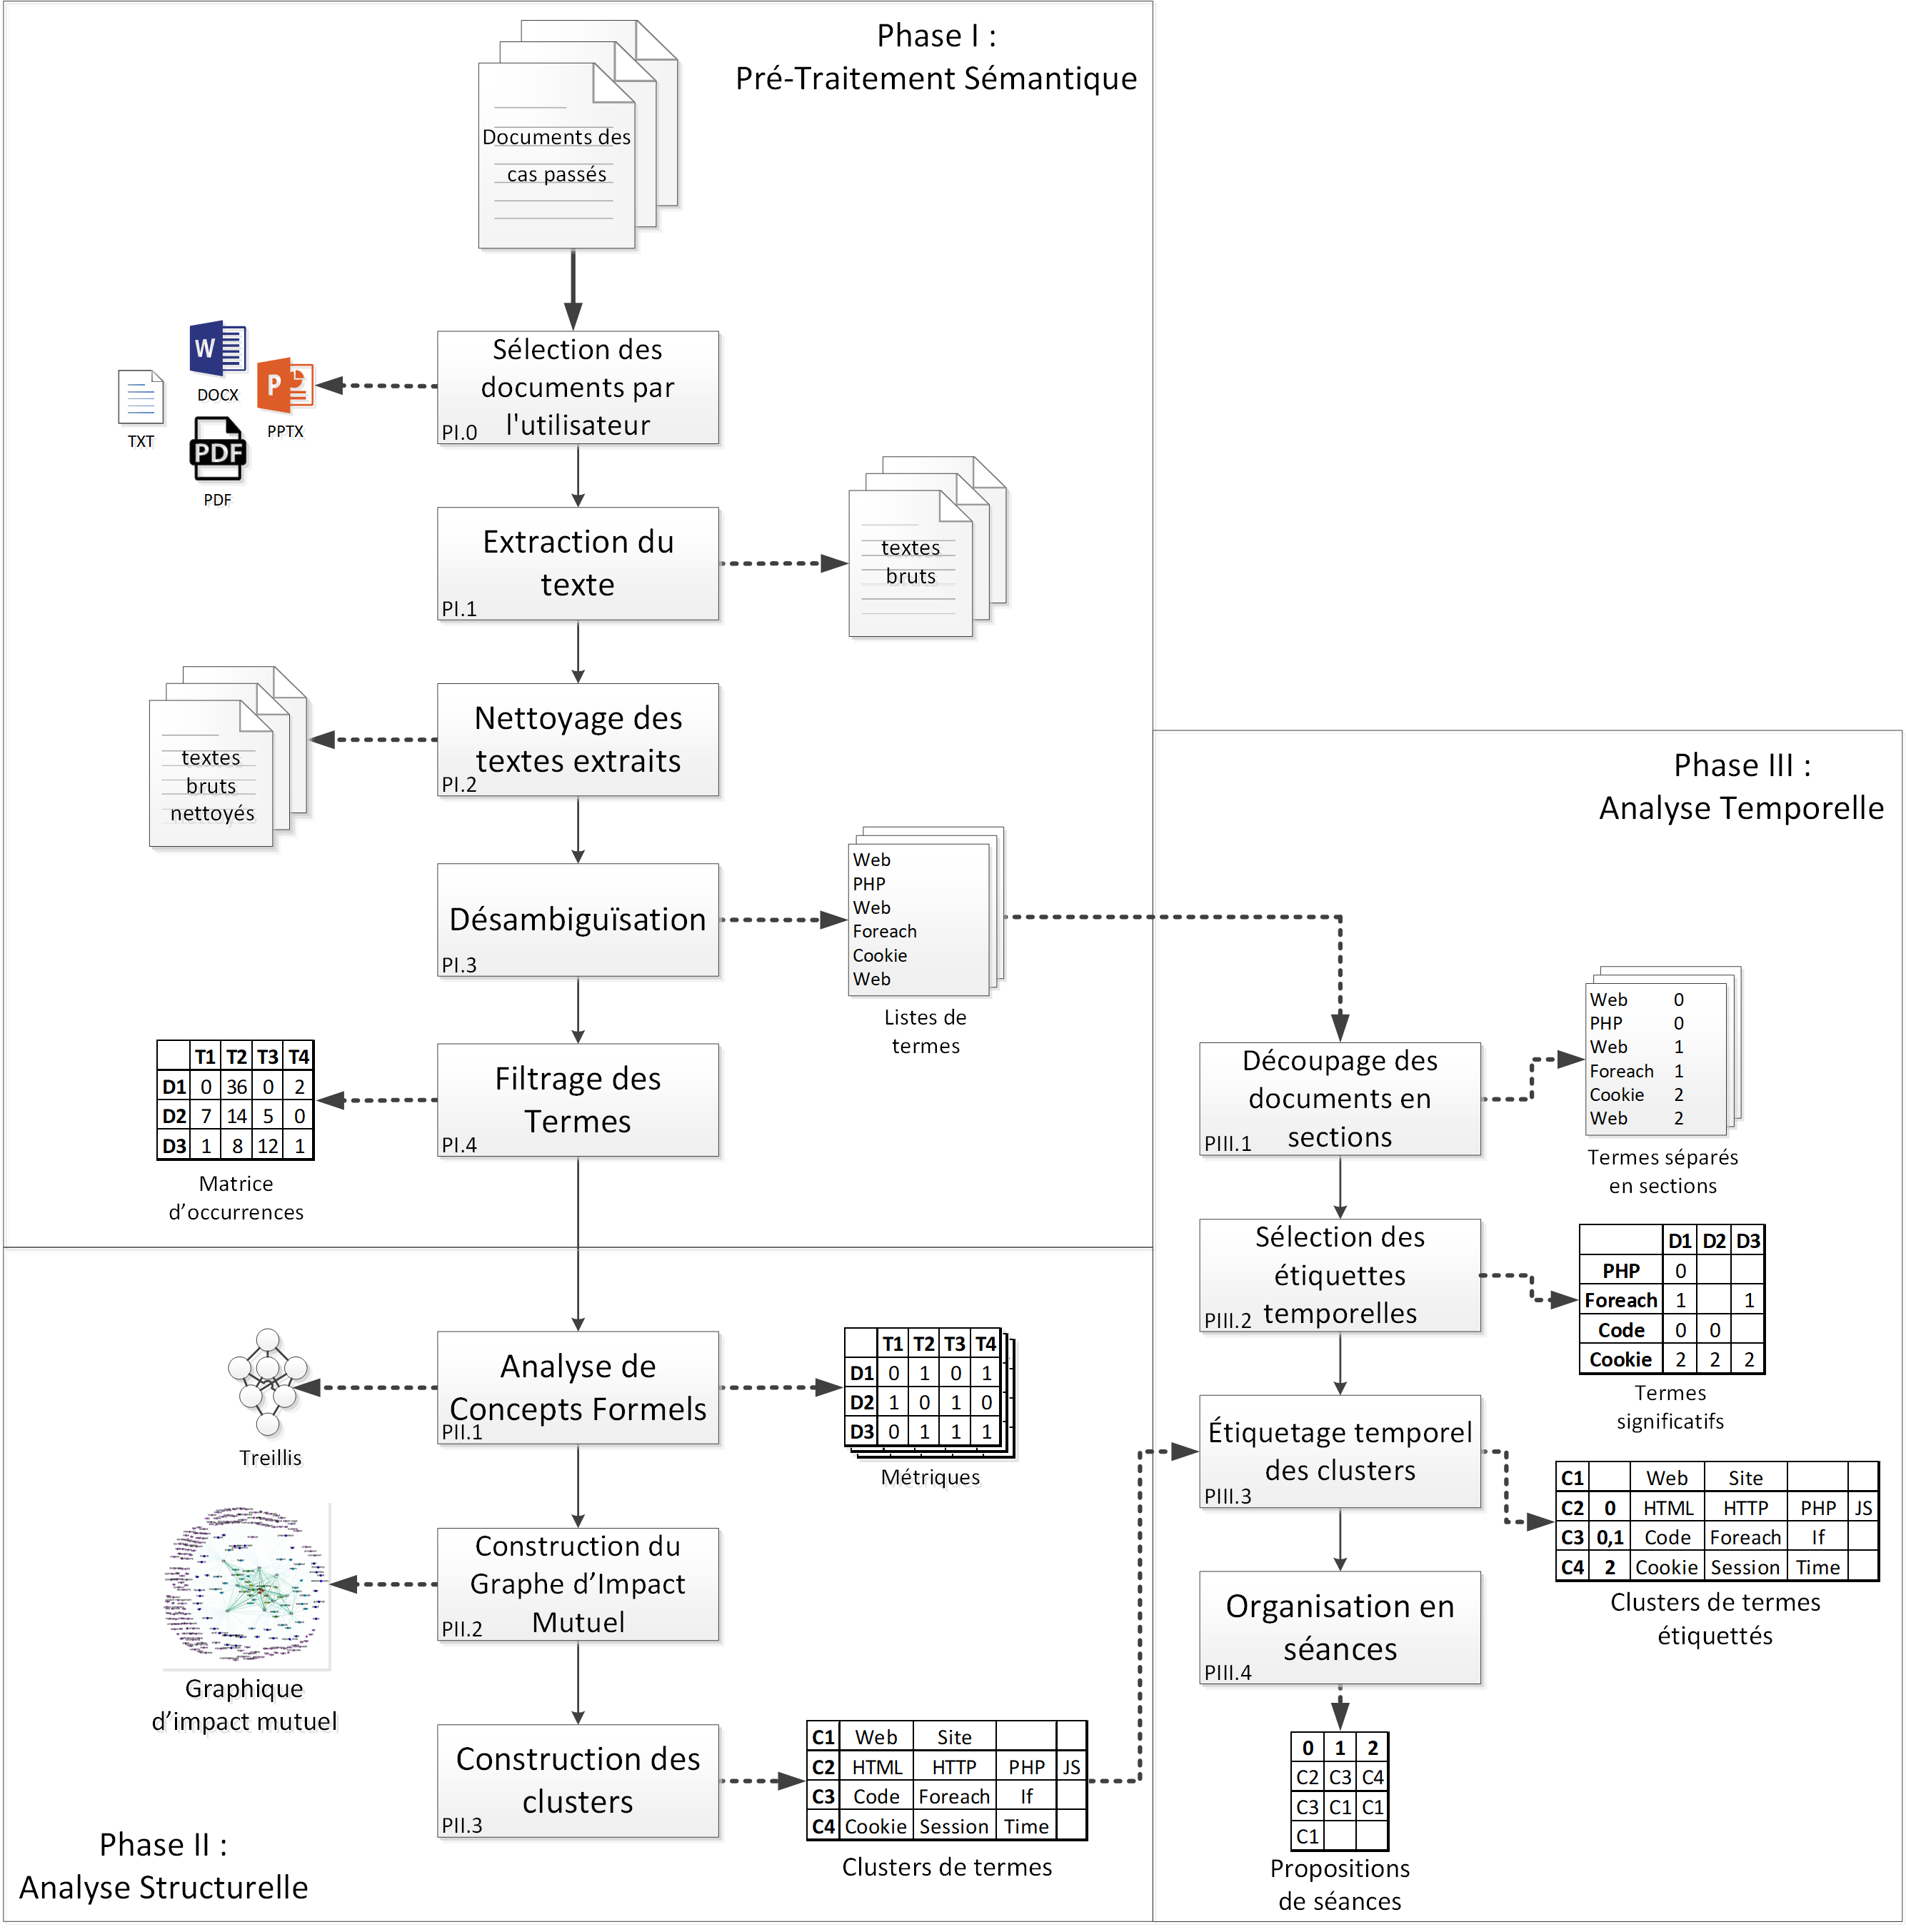
\includegraphics[scale=0.6]{5-Conclusion/images/schema_final+temporel.png}
}
\caption{Détails de la méthode CREA étendue avec l'analyse temporelle}
\label{figure:5-MethodeGeneraleFinale+Temporel}
\end{figure}
%\end{figure*} % Figure flottante
% To use it : fig~\ref{label}

\vfill
\hspace{0pt}
